%  LaTeX support: latex@mdpi.com 
%  For support, please attach all files needed for compiling as well as the log file, and specify your operating system, LaTeX version, and LaTeX editor.

%=================================================================
\documentclass[journal,article,submit,moreauthors]{Definitions/mdpi} 
%\documentclass[preprints,article,submit,moreauthors]{Definitions/mdpi} 
% For posting an early version of this manuscript as a preprint, you may use "preprints" as the journal. Changing "submit" to "accept" before posting will remove line numbers.

% Below journals will use APA reference format:
% admsci, aieduc, behavsci, businesses, econometrics, economies, education, ejihpe, famsci, games, humans, ijcs, ijfs, investment, fclam, jintelligence, journalmedia, jrfm, jsam, languages, opermanag, peacestud, pmh, psycholint, publications, tourismhosp, youth

% Below journals will use Chicago reference format:
% arts, genealogy, histories, humanities, laws, literature, religions, risks, socsci

%--------------------
% Class Options:
%--------------------
%----------
% journal
%----------
% Choose between the following MDPI journals:
% accountaudit, acn, acoustics, actuators, addictions, addictprev, adhesives, adolescents, aerobiology, aerospace, agriculture, agriengineering, agrochemicals, agronomy, ai, aichem, aieng, aimater, aimed, aipa, air, aisens, aisoc, algorithms, allergies, alloys, amh, analog, analytica, analytics, anatomia, anesthres, animals, antibiotics, antibodies, antioxidants, applbiosci, appliedchem, appliedmath, appliedphys, applmech, applmicrobiol, applnano, applsci, aps, aquacj, archaeolstud, architecture, arm, arthropoda, asc, asi, astronautics, astronomy, atmosphere, atoms, audiolres, automation, axioms, bacteria, batteries, bdcc, beverages, biochem, bioengineering, biologics, biology, biomass, biomechanics, biomed, biomedicines, biomedinformatics, biomimetics, biomolecules, biophysica, bioresourbioprod, biosensors, biosphere, biotech, birds, blockchains, bloods, blsf, brainsci, breath, buildings, cancers, carbon, cardio, cardiogenetics, cardiovascmed, catalysts, cells, ceramics, challenges, chemengineering, chemistry, chemosensors, chemproc, children, chips, cimb, civileng, cleantechnol, climate, clinbioenerg, clinpract, clockssleep, cmd, cmtr, coasts, coatings, colloids, colorants, commodities, complexities, complications, compounds, computation, computers, condensedmatter, conservation, constrmater, cosmetics, covid, crops, cryo, cryptography, crystals, csmf, ctn, culture, curroncol, cyber, dairy, data, ddc, dentistry, dermato, dermatopathology, designs, devices, dhi, diabetology, diagnostics, dietetics, digital, disabilities, diseases, diversity, dna, drones, drugreact, drylands, dynamics, earth, ebj, ecm, ecologies, edm, eesp, electricity, electrochem, electronicmat, electronics, embodiedintell, encyclopedia, endocrines, energies, eng, engproc, entomology, entropy, environments, environremediat, epidemiologia, epigenomes, esa, est, fermentation, fibers, fintech, fire, fishes, fluids, foodeng, foods, forecasting, forensicsci, forests, fossstud, foundations, fractalfract, freshwater, fuels, future, futureinternet, futurepharmacol, futurephys, futuretransp, galaxies, gases, gastroent, gastrointestdisord, gastronomy, gels, genes, geochem, geographies, geohazards, geomatics, geometry, geosciences, geotechnics, geriatrics, germs, glacies, grainsci, grasses, green, greenhealth, gucdd, gynecolcancer, hardware, hazardousmatters, healthcare, healthcmater, hearts, hemato, hematolrep, hep, heritage, higheredu, highthroughput, horticulturae, hospitals, hydrobiology, hydrogen, hydrology, hydrometeorology, hydropower, hygiene, idr, iic, ijem, ijerph, ijgi, ijmd, ijms, ijns, ijom, ijp, ijpb, ijt, ijtm, ijtpp, ijtst, ime, immuno, industries, inflammj, informatics, information, infrastructures, inorganics, insects, instruments, inventions, iot, j, jaestheticmed, jal, japma, jcdd, jcm, jcp, jcrm, jcs, jcto, jdad, jdb, jdream, jemr, jeta, jfb, jfmk, jfth, jgbg, jgg, jimaging, jlpea, jmahp, jmmp, jmms, jmp, jmse, jne, jnt, jof, joi, joitmc, joma, jop, joptm, jor, jox, jpbi, jphytomed, jpm, jsan, jtaer, jvd, jzbg, kidneydial, kinasesphosphatases, knowledge, labmed, laboratories, lam, land, lasers, legumes, life, lights, limnolrev, lipidology, liquids, livers, logics, logistics, lubricants, lymphatics, machines, macromol, magnetism, magnetochemistry, make, marinedrugs, maritime, materials, materproc, mathematics, mca, mcb, measurements, medicina, medicines, medsci, membranes, merits, metabolites, metals, meteorology, methane, metrics, metrology, micro, microarrays, microbiolres, microelectronics, micromachines, microorganisms, microplastics, microwave, minerals, mining, mmphys, modelling, molbank, molecules, mollusca, mps, msf, mti, multimedia, muscles, nanoenergyadv, nanomanufacturing, nanomaterials, ncrna, ndt, network, neuroglia, neuroimaging, neurolint, neurosci, nitrogen, notspecified, nursrep, nutraceuticals, nutrients, obesities, occuphealth, oceans, ohbm, onco, optics, oral, organics, organoids, osteology, oxygen, pandemics, parasites, parasitologia, particles, pathogens, pathophysiology, pediatrrep, pets, pharmaceuticals, pharmaceutics, pharmacoepidemiology, pharmacy, phc, philosophies, photochem, photonics, photovoltaics, phycology, physchem, physics, physiologia, plants, plasma, platforms, pollutants, polymers, polysaccharides, populations, poultry, powders, precision, precisoncol, preprints, proceedings, processes, prosthesis, proteomes, psf, psychiatryint, psychoactives, purification, quantumrep, quaternary, qubs, radiation, rareearths, rdt, reactions, realestate, receptors, recycling, regeneration, remotesensing, reports, reprodmed, resources, rheumato, rjpm, robotics, rsee, ruminants, safety, sanpp, sca, sci, scipharm, sclerosis, seeds, sensors, separations, sexes, shi, signals, sinusitis, siuj, skins, smartcities, smartfish, sna, societies, software, soilsystems, solar, solids, spectroscj, sports, standards, stats, std, stratsediment, stresses, strokerep, superintelligence, surfaces, surgeries, suschem, sustainability, sustainfoods, sustainpackag, symmetry, synbio, systems, tae, targets, taxonomy, technologies, telecom, test, textiles, thalassrep, therapeutics, thermo, timespace, tomography, toxics, toxins, tph, transplantology, transportation, traumacare, traumas, tri, tropicalmed, universe, urbansci, uro, vaccines, vehicles, venereology, vetsci, vibration, virtualworlds, viruses, vision, waste, water, welding, wem, wevj, wild, wind, women, world, zoonoticdis

%---------
% article
%---------
% The default type of manuscript is "article", but can be replaced by: 
% abstract, addendum, article, benchmark, book, bookreview, briefcommunication, briefreport, casereport, changes, clinicopathologicalchallenge, comment, commentary, communication, conceptpaper, conferenceproceedings, correction, conferencereport, creative, datadescriptor, discussion, entry, expressionofconcern, extendedabstract, editorial, essay, erratum, fieldguide, hypothesis, interestingimages, letter, meetingreport, monograph, newbookreceived, obituary, opinion, proceedingpaper, projectreport, reply, retraction, review, perspective, protocol, shortnote, studyprotocol, supfile, systematicreview, technicalnote, viewpoint, guidelines, registeredreport, tutorial,  giantsinurology, urologyaroundtheworld
% supfile = supplementary materials

%----------
% submit
%----------
% The class option "submit" will be changed to "accept" by the Editorial Office when the paper is accepted. This will only make changes to the frontpage (e.g., the logo of the journal will get visible), the headings, and the copyright information. Also, line numbering will be removed. Journal info and pagination for accepted papers will also be assigned by the Editorial Office.

%------------------
% moreauthors
%------------------
% If there is only one author the class option oneauthor should be used. Otherwise use the class option moreauthors.

%=================================================================
% MDPI internal commands - do not modify
\firstpage{1} 
\makeatletter 
\setcounter{page}{\@firstpage} 
\makeatother
\pubvolume{1}
\issuenum{1}
\articlenumber{0}
\pubyear{2026}
\copyrightyear{2026}
%\externaleditor{Firstname Lastname} % More than 1 editor, please add `` and '' before the last editor name
\datereceived{ } 
\daterevised{ } % Comment out if no revised date
\dateaccepted{ } 
\datepublished{ } 
%\datecorrected{} % For corrected papers: "Corrected: XXX" date in the original paper.
%\dateretracted{} % For retracted papers: "Retracted: XXX" date in the original paper.
%\doinum{} % Used for some special journals, like molbank
%\pdfoutput=1 % Uncommented for upload to arXiv.org
%\CorrStatement{yes}  % For updates
%\longauthorlist{yes} % For many authors that exceed the left citation part
%\IsAssociation{yes} % For association journals

%=================================================================
% Add packages and commands here. The following packages are loaded in our class file: fontenc, inputenc, calc, indentfirst, fancyhdr, graphicx, epstopdf, lastpage, ifthen, float, amsmath, amssymb, lineno, setspace, enumitem, mathpazo, booktabs, titlesec, etoolbox, tabto, xcolor, colortbl, soul, multirow, microtype, tikz, totcount, changepage, attrib, upgreek, array, tabularx, pbox, ragged2e, tocloft, marginnote, marginfix, enotez, amsthm, natbib, hyperref, cleveref, scrextend, url, geometry, newfloat, caption, draftwatermark, seqsplit

\usepackage{algorithmicx}
\usepackage{algorithm}
\usepackage{algpseudocode}

% cleveref: load \crefname definitions after \begin{document}

%=================================================================
% Please use the following mathematics environments: Theorem, Lemma, Corollary, Proposition, Characterization, Property, Problem, Example, ExamplesandDefinitions, Hypothesis, Remark, Definition, Notation, Assumption
%% For proofs, please use the proof environment (the amsthm package is loaded by the MDPI class).

%=================================================================
% Full title of the paper (Capitalized)
\Title{Search-Trajectory Patterns as Feedback for Adaptive Metaheuristic Configuration Control}

% Author Orchid ID: enter ID or remove command
\newcommand{\orcidauthorA}{0009-0005-4516-2358} % José villamayor
\newcommand{\orcidauthorB}{0009-0001-3259-454X} % watona luca
\newcommand{\orcidauthorC}{0000-0002-0079-3974} % profe ema

% Authors, for the paper (add full first names)
\Author{José Villamayor $^{1}$\orcidA{}, Lucas Erazo $^{1}$\orcidB{}, Ricardo Soto $^{1}$, José Garcia $^{2}$,and Emanuel Vega $^{1,}$*\orcidC{}}


%\longauthorlist{yes}

% MDPI internal command: Authors, for metadata in PDF
\AuthorNames{José Villamayor, Lucas Erazo, Ricardo Soto, José Garcia, and Emanuel Vega}

%\longauthorlist{yes}

% Affiliations / Addresses (Add [1] after \address if there is only one affiliation.)
%\author[2]{\fnm{José} \sur{Garcia}}\email{jose.garcia@pucv.cl}

\address{%
$^{1}$ \quad Escuela de Ingeniería Informática, Pontificia 
 Universidad Católica de Valparaíso, Valparaíso 2362807, Chile; jose.villamayor@pucv.cl (J.V); lucas.erazo@pucv.cl (L.E); ricardo.soto@pucv.cl (R.S) \\
$^{2}$ \quad Escuela de Ingeniería de Construcción y Transporte, Pontificia Universidad Católica de Valparaíso, Valparaíso 2362804, Chile; jose.garcia@pucv.cl (J.G) }

% Contact information of the corresponding author
\corres{Correspondence: emanuel.vega@pucv.cl (E.V)}

% Current address and/or shared authorship
%\firstnote{Current address: Affiliation.}  
% Current address should not be the same as any items in the Affiliation section.

%\secondnote{These authors contributed equally to this work.}
% The commands \thirdnote{} till \eighthnote{} are available for further notes.

%\simplesumm{} % Simple summary

%\conference{} % An extended version of a conference paper

% Abstract (Do not insert blank lines, i.e. \\) 
\abstract{as optimization progresses. However, adaptive decisions are often based on algorithm-specific feedback or simple indicators that provide limited
information about the evolving search dynamics. This work investigates
explicit pattern-based analysis of the search trajectory as a source of
feedback for adaptive configuration control. A trajectory-driven framework
is proposed in which Derivative Dynamic Time Warping (DDTW) analyzes the
recent best-so-far fitness trajectory against reference patterns representing
sustained progress and lack of progress. The resulting information regulates
switching between predefined exploration- and exploitation-oriented parameter
configurations. Two control strategies are introduced: Binary-Simple, which
reacts directly to trajectory evidence associated with a plateau, and
Binary-Complex, which incorporates multiple search conditions, temporal
persistence, and asymmetric switching. The framework is evaluated on nine
Multidimensional Knapsack Problem instances using BPSO, GA, BGWO, and BDE,
with 31 independent runs per condition. Results show that no fixed
configuration consistently dominates across metaheuristics and instances,
while trajectory-driven adaptation provides significant improvements in
multiple experimental conditions. Binary-Complex achieves the best global
mean rank among the four evaluated strategies and significantly outperforms
Binary-Simple in several pairwise comparisons, although the global Friedman
test does not establish statistically significant differences among all
strategies. Moreover, a common trajectory-analysis parameterization produces
different switching behaviors across the evaluated metaheuristics. These
findings support explicit search-trajectory pattern analysis as a viable
feedback mechanism for adaptive configuration control across different
population-based metaheuristics.}

% Keywords
\keyword{Search Trajectory Analysis; Adaptive Configuration Control; Adaptive Parameter Control; Metaheuristics; Derivative Dynamic Time Warping} 

% The fields PACS, MSC, and JEL may be left empty or commented out if not applicable
%\PACS{J0101}
%\MSC{}
%\JEL{}

%%%%%%%%%%%%%%%%%%%%%%%%%%%%%%%%%%%%%%%%%%
% Only for the journal Diversity
%\LSID{\url{http://}}

%%%%%%%%%%%%%%%%%%%%%%%%%%%%%%%%%%%%%%%%%%
% Only for the journal Applied Sciences
%\featuredapplication{Authors are encouraged to provide a concise description of the specific application or a potential application of the work. This section is not mandatory.}
%%%%%%%%%%%%%%%%%%%%%%%%%%%%%%%%%%%%%%%%%%

%%%%%%%%%%%%%%%%%%%%%%%%%%%%%%%%%%%%%%%%%%
% Only for the journal Data
%\dataset{DOI number or link to the deposited data set if the data set is published separately. If the data set shall be published as a supplement to this paper, this field will be filled by the journal editors. In this case, please submit the data set as a supplement.}
%\datasetlicense{License under which the data set is made available (CC0, CC-BY, CC-BY-SA, CC-BY-NC, etc.)}

%%%%%%%%%%%%%%%%%%%%%%%%%%%%%%%%%%%%%%%%%%
% Only for the journal BioTech, Fishes, Neuroimaging and Toxins
%\keycontribution{The breakthroughs or highlights of the manuscript. Authors can write one or two sentences to describe the most important part of the paper.}

%%%%%%%%%%%%%%%%%%%%%%%%%%%%%%%%%%%%%%%%%%
% Only for the journal Encyclopedia
%\encyclopediadef{For entry manuscripts only: please provide a brief overview of the entry title instead of an abstract.}

%%%%%%%%%%%%%%%%%%%%%%%%%%%%%%%%%%%%%%%%%%
% Different journals have different requirements. Please check the specific journal guidelines in the "Instructions for Authors" on the journal's official website.
%\addhighlights{yes}
%\renewcommand{\addhighlights}{%
%
%\noindent This is an optional section, the goal of which is to increase the discoverability and readability of the article via search engines and other scholars. Highlights should not be a copy of the abstract, but a simple overview allowing the reader to quickly and simply find out what the article is about and what can be cited from it. Each of these parts should be up to 2~bullet points.\vspace{3pt}\\
%\textbf{What are the main findings?}
% \begin{itemize}[labelsep=2.5mm,topsep=-3pt]
% \item First bullet.
% \item Second bullet.
% \end{itemize}\vspace{3pt}
%\textbf{What are the implications of the main findings?}
% \begin{itemize}[labelsep=2.5mm,topsep=-3pt]
% \item First bullet.
% \item Second bullet.
% \end{itemize}
%}

%%%%%%%%%%%%%%%%%%%%%%%%%%%%%%%%%%%%%%%%%%
\begin{document}

%%%%%%%%%%%%%%%%%%%%%%%%%%%%%%%%%%%%%%%%%%

\section{Introduction}

Population-based metaheuristics provide flexible search mechanisms for complex optimization problems by iteratively combining diversification of the search space with intensification around promising solutions. Achieving an effective balance between these behaviors is critical, since excessive exploration may slow convergence, whereas excessive exploitation may lead to premature convergence and loss of search diversity \cite{dhiman2026decade,vcrepinvsek2013exploration,zhang2019balancing}. More importantly, the desirable balance is not necessarily constant during an optimization run, where different stages or conditions of the search may benefit from different algorithmic behaviors \cite{vega2021learning,zhang2019balancing}. This dynamic nature of the search has motivated adaptive mechanisms capable of exploiting information generated during optimization to modify search behavior online \cite{aleti2016systematic}.

Adaptive mechanisms have progressively incorporated richer sources of search information, including successful parameter histories \cite{zhang2009jade}, explicit evolutionary-state estimation \cite{zhan2009adaptive}, stagnation-related indicators \cite{liu2024adaptive}, and learning-based feedback \cite{tatsis2023reinforcement}. These developments highlight the relevance of characterizing the ongoing search before deciding how an algorithm should adapt. Nevertheless, many existing mechanisms remain closely coupled to particular metaheuristics, their internal parameters, or specific search indicators, while explicit pattern-based analysis of the search trajectory remains comparatively less explored as a cross-algorithm source of feedback. These observations motivate investigating whether patterns in the temporal evolution of the search trajectory can provide a source of feedback for regulating exploration- and exploitation-oriented configurations across different metaheuristics.

Accordingly, this work proposes a trajectory-driven adaptive configuration-control framework in which Derivative Dynamic Time Warping (DDTW) is employed to analyze patterns in the recent best-so-far fitness trajectory. Rather than independently adapting individual control parameters, each metaheuristic operates between two predefined parameter configurations associated with exploration- and exploitation-oriented search behaviors. Information derived from the DDTW-based trajectory analysis is then used to regulate the transition between these configurations. In this way, DDTW acts as a search-monitoring mechanism within a broader adaptive controller, allowing configuration changes to respond to patterns observed in the evolving fitness trajectory.

The proposed framework is evaluated on the Multidimensional Knapsack Problem
(MKP) using four population-based metaheuristics from different algorithmic
families: Binary Particle Swarm Optimization (BPSO), Genetic Algorithm (GA),
Binary Grey Wolf Optimizer (BGWO), and Binary Differential Evolution (BDE).
For each metaheuristic, two fixed-configuration baselines are considered,
maintaining either exploration- or exploitation-oriented parameters throughout
the search. Two DDTW-driven adaptive variants are then evaluated under the
same experimental conditions. Both employ discrete configuration switching
but differ in controller complexity: Binary-Simple reacts directly to
trajectory evidence associated with a plateau, whereas Binary-Complex
combines multiple trajectory and progress conditions with temporal
persistence and asymmetric switching. This design enables the effect of
trajectory-driven adaptation to be examined across different metaheuristic
paradigms while also assessing whether increased controller complexity
translates into improved optimization performance.

The main contributions of this work are summarized as follows:

\begin{itemize}

\item A trajectory-driven adaptive configuration-control framework that analyzes patterns in the fitness trajectory and uses the resulting information as feedback to regulate exploration and exploitation during the search.

\item A DDTW-based realization of the proposed framework comprising discrete binary adaptation strategies with varying levels of structural complexity, allowing an assessment of different configuration-switching mechanisms.

\item A cross-metaheuristic experimental assessment involving BPSO, GA, BGWO, and BDE, designed to evaluate the applicability of the same trajectory-driven control principle across different discrete population-based optimization paradigms.

\item A controlled comparison against fixed exploration- and exploitation-oriented configurations to quantify the effect of trajectory-driven adaptation and determine whether increased controller complexity translates into improved optimization performance.
\end{itemize}

\section{Related Work}

The performance of evolutionary and swarm-based metaheuristics is strongly influenced by their parameter configuration, since parameters regulate key components of the search process and may substantially affect the resulting optimization behavior. Thus, parameter setting has been recognized as a fundamental issue in evolutionary computation \cite{eiben-1999,talbi-2009}. In the literature, a well-known distinction is made between parameter tuning, where suitable parameter values are determined before the optimization process, and parameter control, where parameter values are modified during execution \cite{talbi2021,huang2019survey}.

Its relevant to illustrate that while parameter tuning seeks a suitable configuration before the search begins, parameter control allows the algorithm to modify its behavior as the optimization process evolves. This distinction is particularly relevant because appropriate parameter values may depend not only on the problem or problem instance, but also on the current stage of the search. In this context, adaptive parameter control exploits feedback obtained from the ongoing optimization process to guide parameter changes \cite{aleti2016systematic}. Different forms of search feedback and adaptation mechanisms have been investigated in the literature \cite{de2021,karafotias2014}, making both the information used to characterize the search and the mechanism that translates such information into adaptation decisions central aspects of adaptive parameter control.

Following this perspective, adaptive parameter-control approaches differ
substantially in the type of search information used to guide their
adaptation decisions. Early contributions already demonstrated the potential
of exploiting information generated during the search for online adaptation.
For instance, JADE uses information associated with successful parameter
values to adapt the scaling factor $F$ and crossover rate $CR$
\cite{zhang2009jade}. This principle was subsequently extended in SHADE,
which incorporates a historical memory of successful parameter settings to
guide the generation of new values of $F$ and $CR$
\cite{tanabe2013success}. Beyond information derived from successful search
outcomes, early adaptive approaches also explored a more explicit
characterization of the current search state using information from the
population itself. A representative example is the adaptive PSO proposed in \cite{zhan2009adaptive}, which estimates the evolutionary state from population-distribution and fitness information, distinguishing among exploration, exploitation,
convergence, and jumping-out states, and adapts the algorithm accordingly. Collectively, these early approaches demonstrate how different forms of information generated during the search can be exploited to characterize search behavior and guide online adaptation.

More recent studies have expanded the range of information used to drive
online adaptation. In \cite{yang2022spatial}, authors explored the spatial distribution of candidate
solutions as an alternative feedback mechanism for adaptive parameter control,
showing that information beyond conventional fitness-based feedback can be
exploited during the search. Learning-based mechanisms
have also been investigated; for instance, Olivares et al. employed
reinforcement learning to dynamically adapt PSO parameters during execution
\cite{olivares2023learning}. Other approaches have focused on detecting
undesirable search conditions, using covariance-based population information
\cite{song2024differential} or stagnation indicators \cite{liu2024adaptive} to characterize search behavior and adapt algorithm parameters accordingly. More recently,
adaptive parameter control has also been investigated in parallel island-based
metaheuristics, where search progress and performance feedback are used to
dynamically adjust algorithm parameters \cite{prado2025parameter}.

Collectively, these studies demonstrate the value of search-generated
information for online adaptation. However, existing mechanisms are commonly
tailored to specific metaheuristics and control parameters, while explicit
pattern-based analysis of the search trajectory remains comparatively less
explored as a cross-algorithm source of feedback. This motivates the
investigation of trajectory-driven mechanisms for adaptive configuration
control across different metaheuristics.

\section{Background}

This section introduces the main elements required to describe the proposed
framework. First, the Multidimensional Knapsack Problem (MKP) is presented as
the optimization problem used for evaluation. Next, the four population-based
metaheuristics considered in this study are briefly characterized. Finally,
Dynamic Time Warping (DTW) and Derivative Dynamic Time Warping (DDTW) are
introduced as the temporal-analysis techniques underlying the trajectory-pattern
analysis developed in the proposed approach.

\subsection{Multidimensional Knapsack Problem}

The Multidimensional Knapsack Problem (MKP) is a classical NP-hard
combinatorial optimization problem in which a subset of items must be selected
to maximize the total profit while satisfying multiple resource constraints.
Given $n$ items, each item $j$ is associated with a profit $p_j$, while
$w_{ij}$ denotes the consumption of resource $i$ by item $j$. Each resource
$i$ has a maximum available capacity $c_i$. The binary decision variable
$x_j$ indicates whether item $j$ is selected. The problem can be formulated
as

\begin{equation}
\begin{aligned}
\max_{\mathbf{x}} \quad
    & \sum_{j=1}^{n} p_j x_j \\
\text{s.t.} \quad
    & \sum_{j=1}^{n} w_{ij}x_j \leq c_i,
      \qquad i=1,\ldots,m, \\
    & x_j \in \{0,1\},
      \qquad j=1,\ldots,n.
\end{aligned}
\end{equation}

The MKP has been extensively studied in combinatorial optimization and
metaheuristics, and several standardized benchmark sets are available for
experimental evaluation. In this work, the benchmark instances introduced
by Chu and Beasley are considered \cite{chu1998genetic}.

\subsection{Population-Based Metaheuristics}

Four population-based metaheuristics from different algorithmic families are
considered in this study: Binary Particle Swarm Optimization (BPSO), Genetic
Algorithm (GA), Binary Grey Wolf Optimizer (BGWO), and Binary Differential
Evolution (BDE). Their inclusion provides different population-update
mechanisms and search dynamics on which the proposed trajectory-driven control
principle can be evaluated. Table~\ref{tab:mhs} summarizes their main
characteristics.

\begin{table}[htbp]
\centering
\caption{Population-based metaheuristics considered in this study.}
\label{tab:mhs}
\begin{tabular}{@{}p{1.6cm} p{2.2cm} p{5.1cm} p{2.7cm}@{}}
\toprule
\textbf{MH} & \textbf{Family} & \textbf{Main search mechanism} &
\textbf{Binary representation} \\
\midrule

BPSO &
Swarm intelligence &
Particle velocities are updated according to inertia, individual experience,
and global swarm information \cite{kennedy1997discrete}. &
Sigmoid transfer function \\

\midrule

GA &
Evolutionary computation &
Candidate solutions evolve through selection, crossover, and mutation
operators \cite{holland1975adaptation,goldberg1989genetic}. &
Native binary representation \\

\midrule

BGWO &
Swarm intelligence &
Candidate solutions update their positions according to the hierarchical
guidance provided by the $\alpha$, $\beta$, and $\delta$ wolves
\cite{mirjalili2014grey,emary2016binary}. &
Transfer-function-based binarization \\

\midrule

BDE &
Evolutionary computation &
New candidate solutions are generated through differential mutation followed
by crossover and selection \cite{storn1997differential,pampara2006binary}. &
Transfer-function-based binarization \\

\bottomrule
\end{tabular}
\end{table}

Although these algorithms differ in their underlying search mechanisms, each
one contains internal parameters that influence the balance between
diversification and intensification. The specific parameters and
exploration- and exploitation-oriented configurations used in this work are
defined later as part of the proposed approach.

\subsection{Dynamic Time Warping and Derivative Dynamic Time Warping}

Dynamic Time Warping (DTW) is a dynamic-programming technique originally
developed for comparing temporal sequences that may exhibit nonlinear
displacements along the time axis \cite{sakoe1978dynamic}. Unlike a direct
point-to-point distance, DTW searches for an alignment between two sequences
while allowing elements from one sequence to be matched with multiple
elements from the other.

Let

\begin{equation}
A = (a_1,a_2,\ldots,a_n)
\end{equation}

and

\begin{equation}
B = (b_1,b_2,\ldots,b_m)
\end{equation}

be two temporal sequences of lengths $n$ and $m$, respectively. DTW constructs
an accumulated-cost matrix $D \in \mathbb{R}^{(n+1)\times(m+1)}$, where
$D[i,j]$ represents the minimum cost required to align the prefixes
$(a_1,\ldots,a_i)$ and $(b_1,\ldots,b_j)$. Using a local distance
$d(a_i,b_j)$, the recurrence relation is

\begin{equation}
D[i,j] =
d(a_i,b_j)
+
\min
\left\{
D[i-1,j],
D[i,j-1],
D[i-1,j-1]
\right\}.
\end{equation}

The boundary conditions are

\begin{equation}
D[0,0]=0,
\qquad
D[i,0]=\infty,
\qquad
D[0,j]=\infty,
\end{equation}

for $i>0$ and $j>0$. In the present formulation, the local squared
Euclidean cost is used,

\begin{equation}
d(a_i,b_j)=(a_i-b_j)^2.
\end{equation}

The final accumulated cost provides a measure of the dissimilarity between
the two sequences under the optimal admissible temporal alignment.

A limitation of conventional DTW is that differences in the absolute
amplitude of two sequences may induce undesirable temporal warpings. To
reduce this effect, Keogh and Pazzani proposed Derivative Dynamic Time
Warping (DDTW), which performs the alignment on estimates of the local
derivatives rather than directly on the original sequence values
\cite{keogh2001derivative}. Hence,

\begin{equation}
\operatorname{DDTW}(A,B)
=
\operatorname{DTW}(A',B'),
\end{equation}

where $A'$ and $B'$ denote derivative representations of the original
sequences.

The use of derivatives shifts the comparison from absolute fitness levels
toward local variations in the temporal evolution of the sequences. In
particular, additive vertical offsets are removed under differentiation,
since for a shifted sequence

\begin{equation}
\widetilde{A}=A+c,
\end{equation}

its derivative satisfies

\begin{equation}
\widetilde{A}'=A'.
\end{equation}

This property is particularly relevant when the objective is to compare the
shape of search trajectories rather than their absolute objective-function
values. To restrict excessive temporal deformation, DTW can additionally be
constrained using a Sakoe--Chiba band \cite{sakoe1978dynamic}. For a
half-width $w$, only matrix cells satisfying

\begin{equation}
|i-j|\leq w
\end{equation}

\noindent are considered during alignment. Classical DTW requires $O(nm)$ time for
sequences of lengths $n$ and $m$. For sequences of comparable length $n$,
this becomes $O(n^2)$, whereas the Sakoe--Chiba restriction reduces the
number of evaluated cells to approximately $O(nw)$.

The proposed approach uses DDTW to compare recent segments of the fitness
trajectory with predefined reference patterns. The construction of these
patterns, the trajectory window, the resulting feedback signal, and its use
for adaptive configuration control are described in
Section~\ref{sec:proposed_approach}.



%%%%%%%%%%%%%%%%%%%%%%%%%%%%%%%%%%%%%%%%%%
\section{Proposed Approach}
\label{sec:proposed_approach}

\subsection{Trajectory-Driven Adaptive Configuration-Control Framework}
\label{sec:framework_arch}

The proposed framework couples three main components: (i) a population-based
metaheuristic responsible for solving the optimization problem, (ii) a
trajectory-analysis module that continuously characterizes the recent
evolution of the search, and (iii) an adaptive controller that translates
the resulting trajectory information into changes in the operating
configuration of the metaheuristic. Figure~\ref{fig:framework} illustrates
the resulting closed-loop architecture.

\begin{figure}[hbtp]
    \centering
    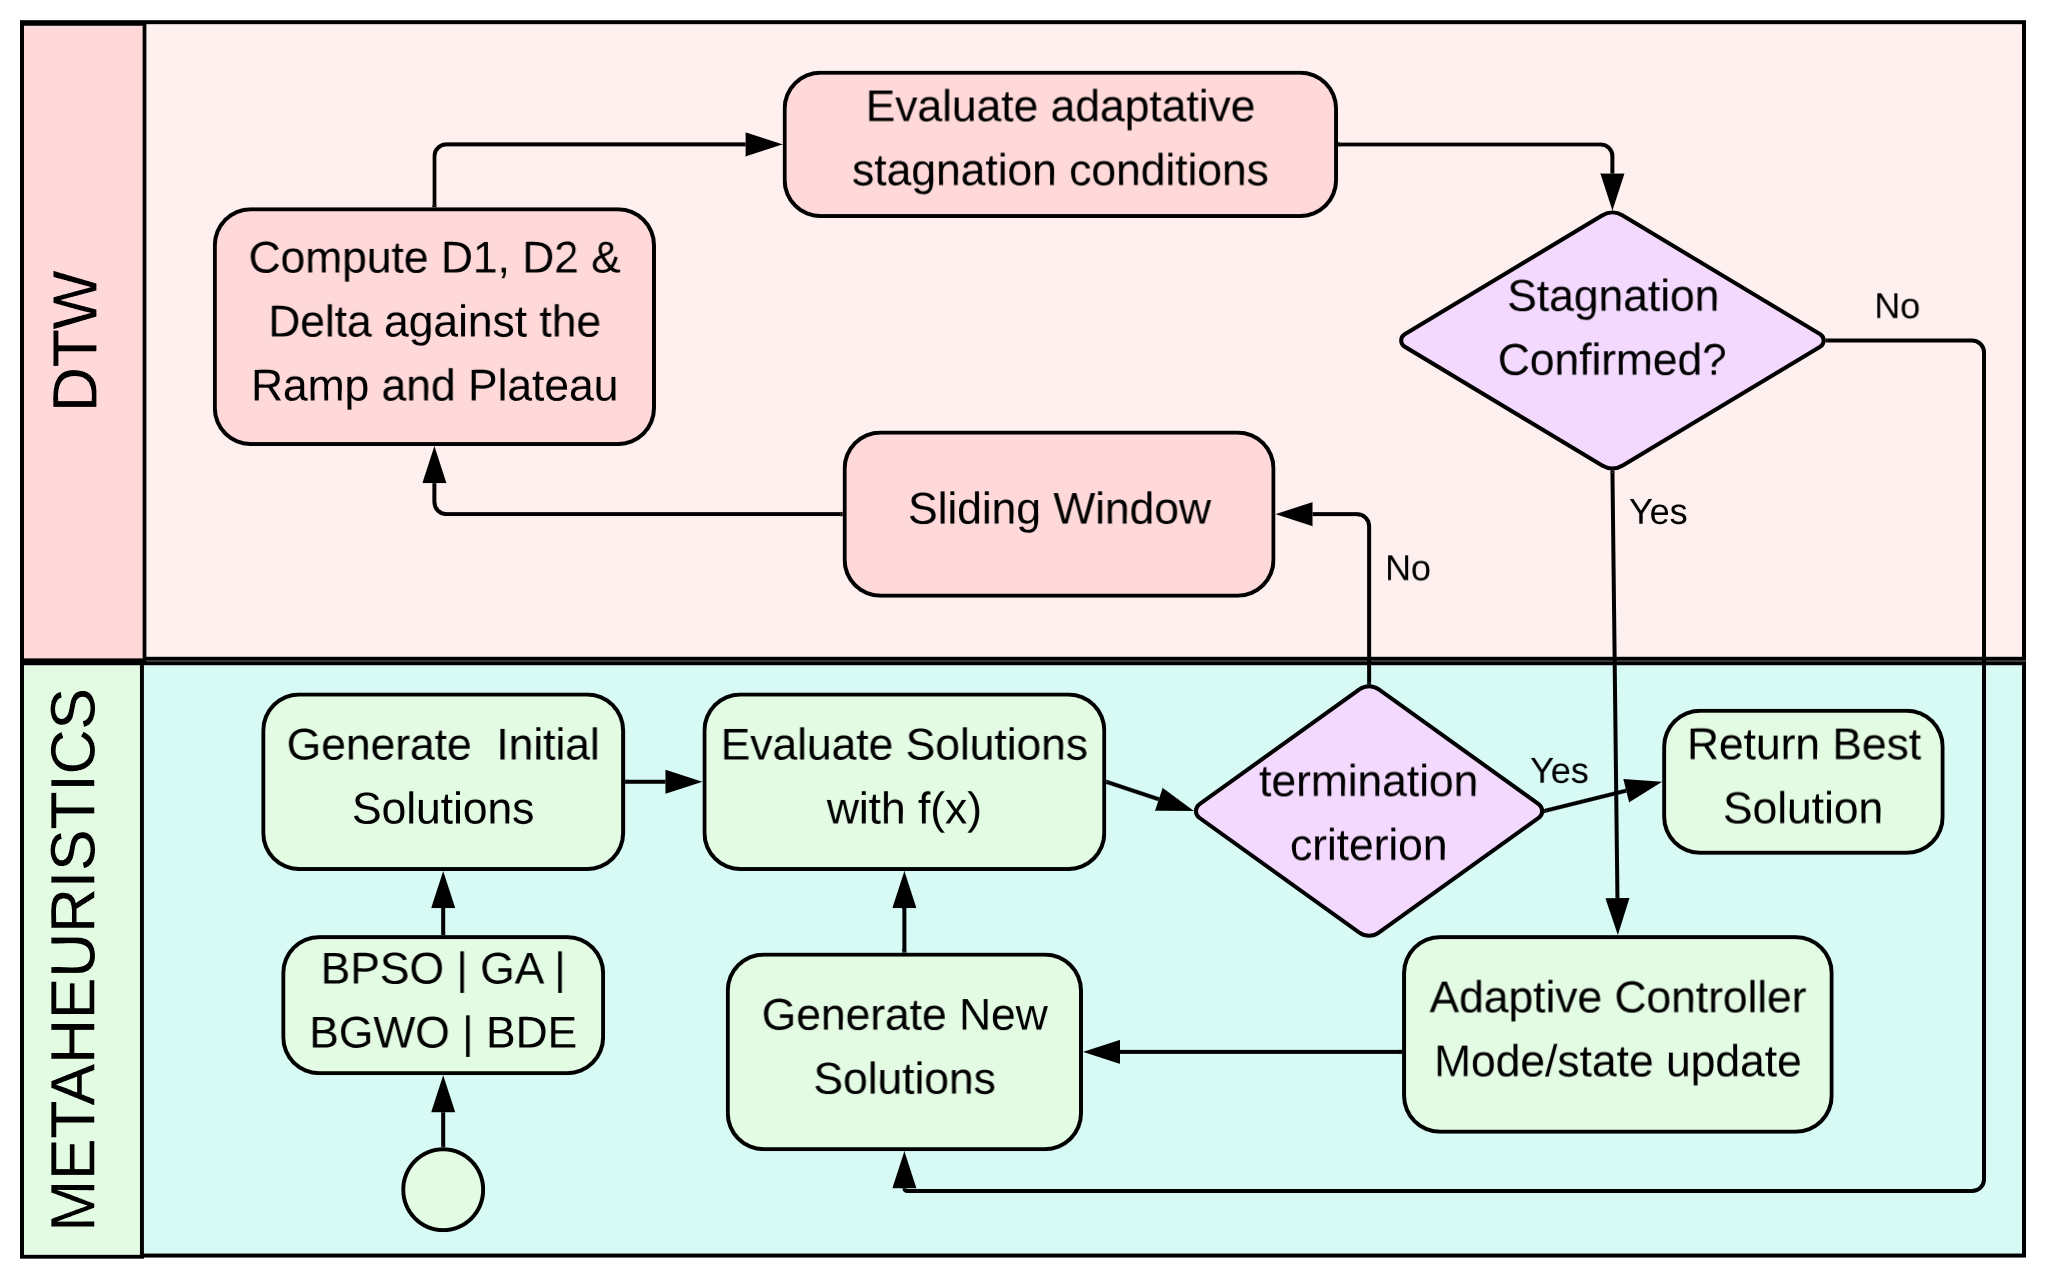
\includegraphics[width=0.88\linewidth]{architecture_diagram.png}
    \caption{Closed-loop architecture of the proposed trajectory-driven adaptive
configuration-control framework.}
    \label{fig:framework}
\end{figure}



At iteration $t$, the metaheuristic evaluates a population of candidate
solutions and records the best-so-far fitness value, denoted by $f_t^*$.
The trajectory-analysis module maintains a sliding window containing the
most recent $W$ observations of this convergence trajectory. During an
initial warm-up period, before a complete window is available, the
metaheuristic operates under its initial configuration. Once $W$
observations have been collected, the trajectory window is compared with
predefined reference patterns representing sustained progress and lack of
progress. The resulting dissimilarity measures are subsequently supplied
to the adaptive controller, which determines the configuration to be used
by the metaheuristic.

The architecture is deliberately modular. The trajectory-analysis module is
independent of the particular update equations of the underlying
metaheuristic, whereas the adaptive controller operates on a common
configuration interface rather than directly on algorithm-specific search
operators. Consequently, the same trajectory information can be processed
by different decision strategies and applied to different metaheuristics by
mapping the resulting control signal to their respective internal
parameters. This separation enables the trajectory-analysis mechanism,
decision logic, and underlying optimization algorithm to be studied under
a common experimental framework.


\subsection{DDTW-Based Trajectory-Pattern Analysis}
\label{sec:trajectory_analysis}

The trajectory-analysis module characterizes the recent search dynamics by
comparing the observed convergence trajectory with predefined geometric
reference patterns. Rather than representing lack of progress exclusively
through the number of consecutive iterations without improvement, the
proposed mechanism evaluates the \emph{shape} of the recent fitness
trajectory using Derivative Dynamic Time Warping (DDTW). The resulting
distances quantify whether the observed search dynamics resemble sustained
progress or a plateau and constitute the feedback information supplied to
the adaptive controller.


\subsubsection{Reference Trajectory Patterns}

Let

\begin{equation}
X_t =
\left(
f_{t-W+1}^*,
f_{t-W+2}^*,
\dots,
f_t^*
\right)
\label{eq:trajectory_window}
\end{equation}

denote the sliding window containing the $W$ most recent best-so-far fitness
values. Two synthetic reference patterns are constructed to represent
contrasting search behaviors.

The first pattern, denoted by $R_t$, represents sustained progress through
a linear trajectory with reference slope $s_{\min}>0$:

\begin{equation}
r_i =
f_{t-W+1}^*
+
s_{\min}(i-1),
\qquad i=1,\ldots,W.
\label{eq:ramp_pattern}
\end{equation}

The second pattern, denoted by $C_t$, represents the absence of progress
through a constant trajectory:

\begin{equation}
c_i =
f_{t-W+1}^*,
\qquad i=1,\ldots,W.
\label{eq:constant_pattern}
\end{equation}

Thus, $R_t$ provides a reference for sustained improvement, whereas $C_t$
represents a fully stagnant trajectory. Since the comparison is performed
on derivative representations through DDTW, the analysis emphasizes the
local evolution of the trajectory rather than its absolute fitness level.


\subsubsection{Trajectory Dissimilarity Measures}

The dissimilarity between the observed trajectory and each reference pattern
is quantified using DDTW with a Sakoe--Chiba constraint of half-width
$w_{\mathrm{SC}}$:

\begin{equation}
D_R(t)
=
\operatorname{DDTW}(X_t,R_t),
\qquad
D_C(t)
=
\operatorname{DDTW}(X_t,C_t).
\label{eq:ddtw_distances}
\end{equation}

A relative trajectory indicator is additionally defined as

\begin{equation}
\Delta_t = D_R(t)-D_C(t).
\label{eq:trajectory_delta}
\end{equation}

Here, $D_R(t)$ measures the dissimilarity between the recent trajectory and
the sustained-progress reference, whereas $D_C(t)$ measures its
dissimilarity from the constant reference. Consequently, $\Delta_t$
provides a relative comparison between both patterns: negative values
indicate that the observed trajectory is closer to the progress reference,
whereas positive values indicate greater similarity to the plateau
reference.


\subsubsection{History-Based Adaptive Thresholds}

Because the magnitude and distribution of the trajectory distances may vary
during the optimization process, the decision thresholds are not defined as
fixed absolute values. Instead, they are dynamically estimated from the
historical distributions of the trajectory metrics.

Let $\mathcal{H}_{R}^{(t)}$, $\mathcal{H}_{C}^{(t)}$, and
$\mathcal{H}_{\Delta}^{(t)}$ denote the accumulated histories of $D_R$,
$D_C$, and $\Delta$ available at iteration $t$, respectively. The adaptive
thresholds are defined as

\begin{equation}
\theta_C(t)
=
\mathcal{P}_{p_{\mathrm{low}}}
\left(\mathcal{H}_{C}^{(t)}\right),
\label{eq:threshold_c}
\end{equation}

\begin{equation}
\theta_R(t)
=
\mathcal{P}_{p_{\mathrm{high}}}
\left(\mathcal{H}_{R}^{(t)}\right),
\label{eq:threshold_r}
\end{equation}

and

\begin{equation}
\theta_{\Delta}(t)
=
\mathcal{P}_{p_{\mathrm{high}}}
\left(\mathcal{H}_{\Delta}^{(t)}\right),
\label{eq:threshold_delta}
\end{equation}

where $\mathcal{P}_{p}(\cdot)$ denotes the $p$-th percentile of the
corresponding historical distribution. The lower percentile
$p_{\mathrm{low}}$ identifies unusually small distances to the plateau
reference, whereas the upper percentile $p_{\mathrm{high}}$ identifies
unusually large deviations from the sustained-progress reference or
correspondingly large values of the relative trajectory indicator.

This history-based formulation allows the decision criteria to adapt to the
distance distributions observed during each optimization run, reducing
their dependence on manually specified absolute distance thresholds.


\subsection{Adaptive Configuration-Control Strategies}
\label{sec:adaptation_strategies}

The trajectory information described above is translated into changes in
the search configuration through two binary adaptive control strategies.
Both strategies operate on the same trajectory information and configuration
interface but differ in the complexity of the decision mechanism used to
trigger transitions between exploration and exploitation.

For binary control, let

\begin{equation}
s_t \in \{0,1\}
\end{equation}

denote the search mode at iteration $t$, where $s_t=0$ selects the
exploitation-oriented configuration and $s_t=1$ selects the
exploration-oriented configuration. The corresponding parameter vector can
be expressed as

\begin{equation}
\boldsymbol{\theta}_t =
\begin{cases}
\boldsymbol{\theta}^{\mathrm{exploit}}, & s_t=0,\\
\boldsymbol{\theta}^{\mathrm{explore}}, & s_t=1,
\end{cases}
\label{eq:binary_config}
\end{equation}

where $\boldsymbol{\theta}^{\mathrm{exploit}}$ and
$\boldsymbol{\theta}^{\mathrm{explore}}$ denote the two predefined
algorithm-specific parameter configurations. Their numerical values for
BPSO, GA, BGWO, and BDE are reported in the Experimental Setup.


\subsubsection{Binary-Simple Strategy}

Binary-Simple constitutes the lowest-complexity trajectory-driven controller.
It uses only the distance to the plateau reference and does not require
temporal persistence of the detected condition. The decision rule is

\begin{equation}
s_t =
\begin{cases}
1, & D_C(t) \leq \theta_C(t),\\
0, & \text{otherwise}.
\end{cases}
\label{eq:binary_simple}
\end{equation}

Therefore, when the recent trajectory becomes unusually similar to the
plateau reference with respect to its historical behavior, the controller
selects the exploration-oriented configuration. Otherwise, the
exploitation-oriented configuration is used.


\subsubsection{Binary-Complex Strategy}

Binary-Complex extends the previous controller by combining multiple
trajectory and progress conditions with temporal persistence and asymmetric
switching. Three conditions are evaluated:

\begin{align}
C_{\mathrm{noimp}}(t) &:\
\ell_{\mathrm{noimp}}(t) \geq \pi_{\max},
\label{eq:cond_noimp}\\
C_{\mathrm{plateau}}(t) &:\
D_C(t) \leq \theta_C(t),
\label{eq:cond_plateau}\\
C_{\mathrm{progress}}(t) &:\
\left[D_R(t) \geq \theta_R(t)\right]
\lor
\left[\Delta_t \geq \theta_{\Delta}(t)\right].
\label{eq:cond_progress}
\end{align}

Here, $\ell_{\mathrm{noimp}}(t)$ denotes the number of consecutive iterations
without improvement in the best-so-far fitness, and $\pi_{\max}$ defines the
minimum number of such iterations required to provide explicit evidence of
lack of progress. The second condition identifies trajectories unusually
close to the plateau reference, whereas the third captures trajectories that
are unusually distant from the sustained-progress pattern, either directly
through $D_R(t)$ or relatively through $\Delta_t$.

Let

\begin{equation}
C_{\mathrm{stag}}(t)
=
C_{\mathrm{noimp}}(t)
\land
C_{\mathrm{plateau}}(t)
\land
C_{\mathrm{progress}}(t)
\label{eq:composite_stagnation}
\end{equation}

denote the composite stagnation condition. A transition from exploitation
to exploration is performed only when $C_{\mathrm{stag}}(t)$ remains
satisfied for $\tau_{\mathrm{pat}}$ consecutive iterations. In contrast, a
strict improvement in the best-so-far fitness immediately returns the
algorithm to the exploitation-oriented configuration:

\begin{equation}
s_t =
\begin{cases}
1,
&
s_{t-1}=0
\;\land\;
C_{\mathrm{stag}}(k)=1
\quad
\forall k\in
\{t-\tau_{\mathrm{pat}}+1,\ldots,t\},
\\[2mm]
0,
&
s_{t-1}=1
\;\land\;
f_t^*>f_{t-1}^*,
\\[2mm]
s_{t-1},
&
\text{otherwise}.
\end{cases}
\label{eq:binary_complex}
\end{equation}

This asymmetric hysteresis requires sustained evidence of stagnation before
activating exploration, thereby reducing sensitivity to transient trajectory
fluctuations. Conversely, once the exploratory configuration produces a
strict improvement in the best-so-far solution, the controller immediately
returns to exploitation so that the newly discovered region can be
intensified.



%%%%%%%%%%%%%%%%%%%%%%%%%%%%%%%%%%%%%%%%%%
\section{Experimental Setup}
\label{sec:experimental_setup}

\subsection{Benchmark Instances and Metaheuristic Configurations}
\label{sec:instances}

The proposed framework is evaluated using benchmark instances from the
Chu--Beasley Multidimensional Knapsack Problem (MKP) test suite
\cite{chu1998genetic}, available through the OR-Library. Nine benchmark
groups are considered, corresponding to the combinations of three numbers
of constraints ($m\in\{5,10,30\}$) and three problem dimensions
($n\in\{100,250,500\}$). The first instance from each group is selected,
resulting in nine evaluation instances. This selection provides a controlled
set covering increasing problem dimensions and constraint levels.
Table~\ref{tab:instances} summarizes their characteristics and known optimal
objective values.

\begin{table}[htbp]
\centering
\caption{MKP benchmark instances considered in the experimental evaluation.}
\label{tab:instances}
\begin{tabular}{@{}l c c r@{}}
\toprule
\textbf{Instance} &
\textbf{Constraints ($m$)} &
\textbf{Items ($n$)} &
\textbf{Known optimum} \\
\midrule
mknapcb1 & 5  & 100 & 24\,381 \\
mknapcb2 & 5  & 250 & 59\,312 \\
mknapcb3 & 5  & 500 & 120\,130 \\
mknapcb4 & 10 & 100 & 23\,064 \\
mknapcb5 & 10 & 250 & 59\,187 \\
mknapcb6 & 10 & 500 & 117\,726 \\
mknapcb7 & 30 & 100 & 21\,946 \\
mknapcb8 & 30 & 250 & 56\,693 \\
mknapcb9 & 30 & 500 & 115\,868 \\
\bottomrule
\end{tabular}
\end{table}

Candidate solutions that violate one or more resource constraints are
restored to feasibility using a greedy repair procedure. Infeasible
solutions are first repaired by iteratively removing low-density items until
all constraints are satisfied. A subsequent insertion phase considers
high-density items and adds them whenever their inclusion preserves
feasibility. The same repair procedure is applied to all metaheuristics and
adaptive variants to avoid introducing algorithm-dependent differences in
constraint handling.


\subsubsection{Metaheuristic Configurations}
\label{sec:mh_config}

All four metaheuristics use a population size of $N=20$ and a computational
budget of $T=2000$ iterations. Each experimental condition is evaluated over
$R=31$ independent runs. These settings are kept fixed across algorithms,
instances, and control strategies.

Four experimental variants are considered for each metaheuristic:
Vanilla-Exploitation, Vanilla-Exploration, Binary-Simple, and Binary-Complex.
The two Vanilla variants maintain a fixed exploitation- or
exploration-oriented parameter configuration throughout the entire run,
whereas Binary-Simple and Binary-Complex dynamically switch between the same
two configurations according to the trajectory-driven control mechanisms
described in Section~\ref{sec:adaptation_strategies}. For BPSO, BGWO, and
BDE, continuous internal quantities are mapped to binary decisions using a
sigmoid transfer function. Table~\ref{tab:mh_params} reports the parameter
values defining the two configurations for each metaheuristic.

\begin{table}[htbp]
\centering
\caption{Exploration- and exploitation-oriented parameter configurations
used for each metaheuristic.}
\label{tab:mh_params}
\begin{tabular}{@{}l l l l@{}}
\toprule
\textbf{MH} &
\textbf{Parameter} &
\textbf{Exploitation} &
\textbf{Exploration} \\
\midrule

\multirow{3}{*}{BPSO}
  & $w$   & 0.729   & 0.9 \\
  & $c_1$ & 1.49445 & 2.5 \\
  & $c_2$ & 1.49445 & 0.5 \\

\midrule

\multirow{2}{*}{GA}
  & $p_c$ & 0.9  & 0.6 \\
  & $p_m$ & 0.01 & 0.15 \\

\midrule

BGWO
  & $a$ & 0.5 & 2.0 \\

\midrule

\multirow{2}{*}{BDE}
  & $F$  & 0.5 & 0.9 \\
  & $CR$ & 0.9 & 0.3 \\

\bottomrule
\end{tabular}
\end{table}

The parameter configurations were defined using established parameter
settings and search-behavior principles reported for the corresponding
metaheuristics \cite{clerc2002particle,goldberg1989genetic,
mirjalili2014grey,storn1997differential}. The exploitation-oriented profiles
favor stronger convergence toward promising regions, whereas the
exploration-oriented profiles modify the corresponding parameters to promote
greater diversification. Specifically, the BPSO exploration profile increases
the inertia and cognitive contribution while reducing the social component;
the GA profile increases the mutation probability while reducing the
crossover probability; the BGWO profile uses a larger value of the
exploration-related coefficient $a$; and the BDE profile increases the
differential scaling factor while reducing the crossover rate. These
configurations are kept unchanged across all benchmark instances.


\subsection{DDTW Trajectory-Analysis and Controller Parameters}
\label{sec:dtw_config}

The DDTW-based trajectory-analysis module and both adaptive controllers use
a common parameterization throughout the complete experimental evaluation.
No instance- or metaheuristic-specific adjustment of these parameters is
performed. Table~\ref{tab:dtw_params} summarizes the corresponding values.

\begin{table}[htbp]
\centering
\caption{Parameters of the DDTW-based trajectory-analysis module and adaptive
controllers.}
\label{tab:dtw_params}
\begin{tabular}{@{}l c l@{}}
\toprule
\textbf{Parameter} & \textbf{Value} & \textbf{Description} \\
\midrule
$W$                  & 200 & Sliding-window length \\
$w_{\mathrm{SC}}$    & 2   & Sakoe--Chiba band half-width \\
$s_{\min}$           & 2.0 & Reference slope for sustained progress \\
$p_{\mathrm{low}}$   & 40  & Percentile defining $\theta_C$ \\
$p_{\mathrm{high}}$  & 60  & Percentile defining $\theta_R$ and $\theta_\Delta$ \\
$\pi_{\max}$         & 5   & Minimum consecutive iterations without improvement \\
$\tau_{\mathrm{pat}}$ & 3  & Persistence required for stagnation confirmation \\
\bottomrule
\end{tabular}
\end{table}

The percentile values $p_{\mathrm{low}}=40$ and
$p_{\mathrm{high}}=60$ are used to dynamically derive the trajectory
thresholds from the historical distributions accumulated during each run.
Binary-Simple uses only the plateau-distance condition
$D_C(t)\leq\theta_C(t)$, whereas Binary-Complex combines the three conditions
defined in Section~\ref{sec:adaptation_strategies} together with the
no-improvement threshold $\pi_{\max}$ and persistence parameter
$\tau_{\mathrm{pat}}$.

The same values of $W$, $w_{\mathrm{SC}}$, $s_{\min}$,
$p_{\mathrm{low}}$, and $p_{\mathrm{high}}$ are used by both adaptive
strategies. Consequently, differences between Binary-Simple and
Binary-Complex arise from their decision logic rather than from different
parameterizations of the underlying trajectory-analysis module.


\subsection{Experimental Protocol}
\label{sec:protocol}

Each experimental run corresponds to the application of one metaheuristic under one configuration-control strategy to a given MKP instance. The same
population size, iteration budget, repair mechanism, and trajectory-analysis
parameters are maintained across the corresponding experimental conditions.
Algorithm~\ref{alg:run} summarizes the procedure for a single independent
run.

\begin{algorithm}[hbtp]
\caption{Procedure for a single independent experimental run.}
\label{alg:run}
\begin{algorithmic}[1]

\Require MKP instance $\mathcal{I}$, metaheuristic $\mathcal{A}$,
controller $\mathcal{E}$, random seed $q$, population size $N$,
iteration budget $T$

\State Initialize the pseudo-random number generator using seed $q$
\State Generate the initial population
$\mathcal{P}\leftarrow\{x_1,\ldots,x_N\}\subset\{0,1\}^{n}$
\State Repair infeasible solutions and evaluate the population
\State Set the best solution as $x^*$ and record its fitness $f^*$
\State Initialize the trajectory-analysis module and the initial parameter
configuration of $\mathcal{A}$

\For{$t=1$ \textbf{to} $T$}

    \State Generate candidate solutions using the current configuration of
    $\mathcal{A}$

    \State Repair infeasible solutions and evaluate the resulting candidates

    \State Update the global best solution $x^*$ and best-so-far fitness $f_t^*$

    \State Append $f_t^*$ to the trajectory history

    \If{the trajectory-analysis module has completed the warm-up period}

        \State Compute the DDTW-based trajectory information

        \State Obtain the control decision
        $s_t \leftarrow \mathcal{E}(D_R(t),D_C(t),\Delta_t,\ldots)$

        \State Set the parameter configuration for the next iteration
        according to $s_t$
        ($0\rightarrow$ exploitation, $1\rightarrow$ exploration)

    \EndIf

    \State Store convergence, trajectory-analysis, and controller-state
diagnostics

\EndFor

\State \Return $x^*$, $f_T^*$, and the recorded execution histories

\end{algorithmic}
\end{algorithm}

\section{Results}
\label{sec:results}

This section presents the experimental results obtained for the four
metaheuristics (BPSO, GA, BGWO, and BDE) across the nine MKP benchmark
instances. The analysis considers three complementary aspects: solution
quality, statistical evidence, and computational overhead. In addition,
the switching behavior of the adaptive controllers is examined to provide
insight into how the trajectory-driven mechanisms operate during the search.
Each experimental condition comprises $R=31$ independent runs.

% ============================================================
\subsection{Solution Quality}
\label{subsec:solution_quality}

Optimization performance is first assessed using the final best-so-far
objective values obtained over the independent runs. For each experimental
condition, the best fitness value ($f_{\mathrm{best}}$), mean final fitness
($\bar{f}$), standard deviation ($\sigma$), and relative optimality gap are
reported. Since the global optimum $f^*$ is known for all benchmark
instances, the mean relative optimality gap is computed as

\begin{equation}
    \text{Gap}(\%) =
    \left(
    \frac{f^*-\bar{f}}{f^*}
    \right)\times100.
    \label{eq:gap_results}
\end{equation}

Lower Gap values therefore indicate better average solution quality, with
$\text{Gap}=0$ corresponding to the known optimum.

To provide a concise view of the results in the main text,
Tables~\ref{tab:calidad_mknapcb1},
\ref{tab:calidad_mknapcb5}, and
\ref{tab:calidad_mknapcb9} present three representative instances spanning
increasing problem dimensions and constraint levels:
\texttt{mknapcb1} ($n=100$, $m=5$),
\texttt{mknapcb5} ($n=250$, $m=10$), and
\texttt{mknapcb9} ($n=500$, $m=30$).
The complete results for the remaining six instances are provided in
Appendix~\ref{sec:appendix_tables}.

% --- Representative Instance 1 ---
\begin{table}[htbp]
  \centering
  \small
  \caption{Solution quality on \textbf{mknapcb1}
  ($n=100$, $m=5$, $f^*=24\,381$).}
  \label{tab:calidad_mknapcb1}
  \begin{tabular}{lrrrr}
    \toprule
    \textbf{MH -- Variant} &
    \textbf{Best Fitness} &
    \textbf{Average} &
    \textbf{Std.} &
    \textbf{Gap (\%)} \\
    \midrule
    BPSO -- Vanilla Exploitation & \textbf{24381} & 24256.58 & 46.29 & 0.51 \\
    BPSO -- Vanilla Exploration  & \textbf{24381} & \textbf{24343.65} & 26.75 & \textbf{0.15} \\
    BPSO -- Binary-Simple        & \textbf{24381} & 24329.74 & 32.18 & 0.21 \\
    BPSO -- Binary-Complex       & \textbf{24381} & 24330.87 & 32.34 & 0.21 \\
    \midrule
    GA -- Vanilla Exploitation   & 24373 & 24283.26 & 55.41 & 0.40 \\
    GA -- Vanilla Exploration    & \textbf{24381} & 24309.35 & 31.09 & 0.29 \\
    GA -- Binary-Simple          & 24373 & 24307.23 & 36.21 & 0.30 \\
    GA -- Binary-Complex         & \textbf{24381} & \textbf{24316.90} & 38.86 & \textbf{0.26} \\
    \midrule
    BGWO -- Vanilla Exploitation & 24259 & \textbf{24197.77} & 33.65 & \textbf{0.75} \\
    BGWO -- Vanilla Exploration  & \textbf{24327} & 24190.19 & 38.87 & 0.78 \\
    BGWO -- Binary-Simple        & \textbf{24327} & 24181.58 & 52.96 & 0.82 \\
    BGWO -- Binary-Complex       & \textbf{24327} & 24191.71 & 36.68 & 0.78 \\
    \midrule
    BDE -- Vanilla Exploitation  & 24330 & 24234.52 & 79.08 & 0.60 \\
    BDE -- Vanilla Exploration   & \textbf{24381} & \textbf{24322.32} & 30.15 & \textbf{0.24} \\
    BDE -- Binary-Simple         & \textbf{24381} & 24306.39 & 41.38 & 0.31 \\
    BDE -- Binary-Complex        & 24337 & 24288.06 & 27.59 & 0.38 \\
    \bottomrule
  \end{tabular}
\end{table}

% --- Representative Instance 5 ---
\begin{table}[htbp]
  \centering
  \small
  \caption{Solution quality on \textbf{mknapcb5}
  ($n=250$, $m=10$, $f^*=59\,187$).}
  \label{tab:calidad_mknapcb5}
  \begin{tabular}{lrrrr}
    \toprule
    \textbf{MH -- Variant} &
    \textbf{Best Fitness} &
    \textbf{Average} &
    \textbf{Std.} &
    \textbf{Gap (\%)} \\
    \midrule
    BPSO -- Vanilla Exploitation & 58285 & 57676.74 & 207.82 & 2.55 \\
    BPSO -- Vanilla Exploration  & \textbf{58564} & \textbf{58288.10} & 109.54 & \textbf{1.52} \\
    BPSO -- Binary-Simple        & 58527 & 58224.81 & 148.57 & 1.63 \\
    BPSO -- Binary-Complex       & 58439 & 58186.45 & 123.58 & 1.69 \\
    \midrule
    GA -- Vanilla Exploitation   & \textbf{59094} & \textbf{58830.06} & 130.21 & \textbf{0.60} \\
    GA -- Vanilla Exploration    & 58573 & 58206.61 & 144.26 & 1.66 \\
    GA -- Binary-Simple          & 58966 & 58617.29 & 193.96 & 0.96 \\
    GA -- Binary-Complex         & 58947 & 58690.10 & 152.55 & 0.84 \\
    \midrule
    BGWO -- Vanilla Exploitation & \textbf{58148} & \textbf{57569.81} & 187.46 & \textbf{2.73} \\
    BGWO -- Vanilla Exploration  & 57747 & 57468.90 & 128.10 & 2.90 \\
    BGWO -- Binary-Simple        & 58058 & 57532.39 & 183.26 & 2.80 \\
    BGWO -- Binary-Complex       & 57747 & 57464.65 & 147.07 & 2.91 \\
    \midrule
    BDE -- Vanilla Exploitation  & 58807 & 58394.58 & 193.71 & 1.34 \\
    BDE -- Vanilla Exploration   & 58938 & 58628.68 & 139.05 & 0.94 \\
    BDE -- Binary-Simple         & \textbf{58971} & 58671.94 & 156.25 & 0.87 \\
    BDE -- Binary-Complex        & 58961 & \textbf{58747.71} & 111.18 & \textbf{0.74} \\
    \bottomrule
  \end{tabular}
\end{table}

% --- Representative Instance 9 ---
\begin{table}[htbp]
  \centering
  \small
  \caption{Solution quality on \textbf{mknapcb9}
  ($n=500$, $m=30$, $f^*=115\,868$).}
  \label{tab:calidad_mknapcb9}
  \begin{tabular}{lrrrr}
    \toprule
    \textbf{MH -- Variant} &
    \textbf{Best Fitness} &
    \textbf{Average} &
    \textbf{Std.} &
    \textbf{Gap (\%)} \\
    \midrule
    BPSO -- Vanilla Exploitation & 111723 & 111259.61 & 268.02 & 3.98 \\
    BPSO -- Vanilla Exploration  & \textbf{112766} & \textbf{112194.90} & 248.78 & \textbf{3.17} \\
    BPSO -- Binary-Simple        & 112527 & 112177.81 & 230.27 & 3.18 \\
    BPSO -- Binary-Complex       & 112752 & 112155.48 & 284.79 & 3.20 \\
    \midrule
    GA -- Vanilla Exploitation   & \textbf{115205} & \textbf{114841.97} & 207.64 & \textbf{0.89} \\
    GA -- Vanilla Exploration    & 112886 & 112113.00 & 327.65 & 3.24 \\
    GA -- Binary-Simple          & 114665 & 113450.29 & 579.15 & 2.09 \\
    GA -- Binary-Complex         & 114647 & 114272.58 & 244.37 & 1.38 \\
    \midrule
    BGWO -- Vanilla Exploitation & 111836 & 111465.45 & 183.47 & 3.80 \\
    BGWO -- Vanilla Exploration  & 111784 & 111389.61 & 166.71 & 3.87 \\
    BGWO -- Binary-Simple        & \textbf{111960} & \textbf{111484.71} & 210.11 & \textbf{3.78} \\
    BGWO -- Binary-Complex       & 111803 & 111412.16 & 209.34 & 3.85 \\
    \midrule
    BDE -- Vanilla Exploitation  & 113731 & 112748.32 & 449.92 & 2.69 \\
    BDE -- Vanilla Exploration   & 113456 & 112854.19 & 298.97 & 2.60 \\
    BDE -- Binary-Simple         & \textbf{114342} & 113489.10 & 381.88 & 2.05 \\
    BDE -- Binary-Complex        & 114152 & \textbf{113496.81} & 334.71 & \textbf{2.05} \\
    \bottomrule
  \end{tabular}
\end{table}

The results reveal that the relative performance of the four variants depends
on both the underlying metaheuristic and the benchmark instance. Consequently,
no single fixed configuration consistently dominates across all experimental
conditions.

For BPSO, the exploration-oriented configuration generally provides stronger
performance than the fixed exploitation profile as problem size increases.
On \texttt{mknapcb5}, Vanilla-Exploration achieves a mean gap of $1.52\%$,
compared with $2.55\%$ for Vanilla-Exploitation, while Binary-Simple and
Binary-Complex remain close to the exploration-oriented baseline, with gaps
of $1.63\%$ and $1.69\%$, respectively. A similar pattern is observed on
\texttt{mknapcb9}, where Vanilla-Exploration, Binary-Simple, and
Binary-Complex obtain gaps of $3.17\%$, $3.18\%$, and $3.20\%$,
respectively, compared with $3.98\%$ for Vanilla-Exploitation. Thus, the
adaptive variants avoid the comparatively weaker behavior of the fixed
exploitation profile on these larger BPSO instances while remaining
competitive with the stronger fixed configuration.

GA exhibits a different pattern. Vanilla-Exploitation performs particularly
well on the larger representative instances, achieving gaps of $0.60\%$ on
\texttt{mknapcb5} and $0.89\%$ on \texttt{mknapcb9}. Binary-Complex obtains
the strongest performance among the remaining variants on both instances,
with gaps of $0.84\%$ and $1.38\%$, respectively, but does not surpass the
favorable fixed exploitation configuration. At the same time, Binary-Complex
substantially improves upon Vanilla-Exploration on \texttt{mknapcb9},
reducing the mean gap from $3.24\%$ to $1.38\%$. These results illustrate
that the effectiveness of adaptive control depends on the behavior of the
underlying metaheuristic and that a favorable fixed configuration can remain
difficult to outperform in specific conditions.

For BGWO, differences among the four variants are comparatively small.
On \texttt{mknapcb5}, mean gaps range from $2.73\%$ to $2.91\%$, whereas
on \texttt{mknapcb9} they range from $3.78\%$ to $3.87\%$. Binary-Simple
achieves the lowest mean gap on \texttt{mknapcb9}, while
Vanilla-Exploitation performs best on \texttt{mknapcb5}. The comparatively
narrow performance range suggests that configuration changes have a more
limited effect on BGWO under the evaluated conditions.

The clearest benefits of trajectory-driven adaptation among the
representative instances are observed for BDE. On \texttt{mknapcb5},
Binary-Complex achieves the lowest mean gap ($0.74\%$), improving upon
Vanilla-Exploitation ($1.34\%$), Vanilla-Exploration ($0.94\%$), and
Binary-Simple ($0.87\%$). On \texttt{mknapcb9}, both adaptive strategies
achieve a gap of approximately $2.05\%$, compared with $2.69\%$ and
$2.60\%$ for Vanilla-Exploitation and Vanilla-Exploration, respectively.
This behavior indicates that BDE benefits particularly from dynamically
alternating between the two predefined configurations under the proposed
trajectory-driven control mechanism.

Overall, the descriptive results support two main observations. First, the
preferred fixed configuration varies across metaheuristics and benchmark
conditions, reinforcing the motivation for online configuration control
rather than reliance on a single predefined search profile. Second, the
trajectory-driven variants remain competitive across the evaluated
conditions and provide clear improvements in several cases, particularly
for BDE and for GA when compared with its exploration-oriented baseline.
The following statistical analysis examines whether these observed
differences are supported by inferential evidence.


% ============================================================
\subsection{Statistical Analysis}
\label{subsec:statistical_analysis}

A non-parametric statistical analysis was conducted to complement the
descriptive comparison of solution quality. Two complementary levels of
analysis were considered. First, pairwise comparisons were performed between
Binary-Complex and each of the three alternative strategies:
Vanilla-Exploitation, Vanilla-Exploration, and Binary-Simple. Second, a
Friedman test was used to examine the overall ranking of the four strategies
across the complete set of metaheuristic--instance combinations.

For the pairwise analysis, the Wilcoxon signed-rank test was applied at a
significance level of $\alpha=0.05$. The comparison focuses on
Binary-Complex because it represents the complete trajectory-driven
controller, whereas Binary-Simple provides a lower-complexity adaptive
reference and the two Vanilla variants represent the corresponding fixed
configuration baselines.

% --- Non-Parametric Wilcoxon Signed-Rank Test Table ---
\begin{table*}[htbp]
  \centering
  \small
  \caption{Pairwise Wilcoxon Signed-Rank Test: Proposed \textbf{Binary-Complex} vs. Baselines ($\alpha=0.05$, $R=31$). Verdict signs: $+$ indicates Binary-Complex is statistically superior ($p < 0.05$); $\approx$ indicates no significant difference ($p \ge 0.05$); $-$ indicates baseline is superior.}
  \label{tab:wilcoxon_tests}
  \begin{tabular*}{\textwidth}{@{\extracolsep{\fill}}llcccccc@{}}
    \toprule
    & & \multicolumn{2}{c}{\textbf{vs. Vanilla (Exploit)}} & \multicolumn{2}{c}{\textbf{vs. Vanilla (Explore)}} & \multicolumn{2}{c}{\textbf{vs. Binary-Simple}} \\
    \cmidrule(lr){3-4} \cmidrule(lr){5-6} \cmidrule(lr){7-8}
    \textbf{Instance} & \textbf{Algorithm} & $p$-value & Sign & $p$-value & Sign & $p$-value & Sign \\
    \midrule
    \textbf{mknapcb1}  & BPSO  & 5.726e-06 & $+$ & 0.1610 & $\approx$ & 0.8373 & $\approx$ \\
                       & GA    & 0.0161 & $+$ & 0.2219 & $\approx$ & 0.1261 & $\approx$ \\
                       & BGWO  & 0.3719 & $\approx$ & 0.7220 & $\approx$ & 0.1846 & $\approx$ \\
                       & BDE   & 0.0036 & $+$ & 5.621e-05 & $-$ & 0.0875 & $\approx$ \\
    \midrule
    \textbf{mknapcb2}  & BPSO  & 9.313e-10 & $+$ & 0.0699 & $\approx$ & 0.6883 & $\approx$ \\
                       & GA    & 1.494e-04 & $-$ & 1.173e-06 & $+$ & 0.0063 & $+$ \\
                       & BGWO  & 0.0571 & $\approx$ & 0.8303 & $\approx$ & 0.2473 & $\approx$ \\
                       & BDE   & 1.863e-09 & $+$ & 2.882e-04 & $+$ & 0.3777 & $\approx$ \\
    \midrule
    \textbf{mknapcb3}  & BPSO  & 9.313e-10 & $+$ & 0.0168 & $-$ & 0.5168 & $\approx$ \\
                       & GA    & 6.941e-05 & $-$ & 9.313e-10 & $+$ & 1.863e-09 & $+$ \\
                       & BGWO  & 0.1795 & $\approx$ & 0.2548 & $\approx$ & 0.5481 & $\approx$ \\
                       & BDE   & 9.313e-10 & $+$ & 4.005e-08 & $+$ & 0.8092 & $\approx$ \\
    \midrule
    \textbf{mknapcb4}  & BPSO  & 1.131e-04 & $+$ & 0.1474 & $\approx$ & 0.1554 & $\approx$ \\
                       & GA    & 0.1442 & $\approx$ & 0.6894 & $\approx$ & 0.9273 & $\approx$ \\
                       & BGWO  & 0.8589 & $\approx$ & 0.7764 & $\approx$ & 0.5595 & $\approx$ \\
                       & BDE   & 0.0039 & $+$ & 0.6808 & $\approx$ & 0.2794 & $\approx$ \\
    \midrule
    \textbf{mknapcb5}  & BPSO  & 2.111e-06 & $+$ & 7.148e-04 & $-$ & 0.5566 & $\approx$ \\
                       & GA    & 6.047e-04 & $-$ & 1.174e-06 & $+$ & 0.2396 & $\approx$ \\
                       & BGWO  & 0.0192 & $-$ & 0.8552 & $\approx$ & 0.1763 & $\approx$ \\
                       & BDE   & 2.818e-06 & $+$ & 0.0024 & $+$ & 0.0187 & $+$ \\
    \midrule
    \textbf{mknapcb6}  & BPSO  & 1.863e-09 & $+$ & 0.0037 & $-$ & 0.8141 & $\approx$ \\
                       & GA    & 6.562e-06 & $-$ & 1.733e-06 & $+$ & 1.024e-07 & $+$ \\
                       & BGWO  & 7.017e-04 & $-$ & 0.0875 & $\approx$ & 0.3369 & $\approx$ \\
                       & BDE   & 4.742e-06 & $+$ & 5.960e-07 & $+$ & 0.8754 & $\approx$ \\
    \midrule
    \textbf{mknapcb7}  & BPSO  & 0.0344 & $+$ & 0.1471 & $\approx$ & 0.0157 & $+$ \\
                       & GA    & 1.866e-06 & $+$ & 0.3008 & $\approx$ & 1.0000 & $\approx$ \\
                       & BGWO  & 0.7930 & $\approx$ & 0.5527 & $\approx$ & 0.2076 & $\approx$ \\
                       & BDE   & 1.790e-05 & $+$ & 0.1918 & $\approx$ & 0.8012 & $\approx$ \\
    \midrule
    \textbf{mknapcb8}  & BPSO  & 1.863e-09 & $+$ & 0.4389 & $\approx$ & 0.2133 & $\approx$ \\
                       & GA    & 6.499e-04 & $-$ & 1.733e-06 & $+$ & 0.0052 & $+$ \\
                       & BGWO  & 0.9154 & $\approx$ & 0.2586 & $\approx$ & 0.0267 & $+$ \\
                       & BDE   & 1.968e-05 & $+$ & 0.0014 & $+$ & 0.1701 & $\approx$ \\
    \midrule
    \textbf{mknapcb9}  & BPSO  & 9.313e-10 & $+$ & 0.9397 & $\approx$ & 0.8677 & $\approx$ \\
                       & GA    & 9.313e-10 & $-$ & 9.313e-10 & $+$ & 7.195e-06 & $+$ \\
                       & BGWO  & 0.5115 & $\approx$ & 0.7509 & $\approx$ & 0.2724 & $\approx$ \\
                       & BDE   & 2.560e-06 & $+$ & 1.276e-07 & $+$ & 0.9001 & $\approx$ \\
    \midrule
    \multicolumn{2}{l}{\textbf{Total ($+ / \approx / -$)}} & \multicolumn{2}{c}{\textbf{20 / 8 / 8}} & \multicolumn{2}{c}{\textbf{12 / 20 / 4}} & \multicolumn{2}{c}{\textbf{8 / 28 / 0}} \\
    \bottomrule
  \end{tabular*}
  \vspace{1ex}
\end{table*}

Table~\ref{tab:wilcoxon_tests} summarizes the pairwise results across the
36 metaheuristic--instance combinations. Against Vanilla-Exploitation,
Binary-Complex obtains 20 statistically significant favorable comparisons,
8 cases in which no statistically significant difference is detected, and
8 unfavorable comparisons. The unfavorable cases are concentrated mainly
in GA and BGWO, whereas Binary-Complex exhibits particularly consistent
advantages over the exploitation-oriented baseline for BPSO and BDE.

Against Vanilla-Exploration, Binary-Complex obtains 12 statistically
significant favorable comparisons, 20 cases without a statistically
significant difference, and 4 unfavorable comparisons. This result is
particularly relevant because the exploration-oriented baseline is itself
competitive for several BPSO and BDE instances. Thus, Binary-Complex is
frequently able to match this favorable fixed configuration while producing
significant improvements in a subset of the evaluated conditions.

The direct comparison between the two adaptive strategies provides further
evidence regarding controller complexity. Binary-Complex obtains 8
statistically significant favorable comparisons against Binary-Simple,
while no statistically significant difference is detected in the remaining
28 cases. No statistically significant unfavorable comparison is observed.
The improvements occur in several GA instances and selected BPSO, BGWO, and
BDE conditions, indicating that the additional search conditions, temporal
persistence, and asymmetric switching incorporated into Binary-Complex can
provide measurable benefits over the simpler reactive controller.

It is important to emphasize that the absence of a statistically significant
difference should not be interpreted as statistical equivalence. Rather,
these cases indicate that the available samples do not provide sufficient
evidence to reject the null hypothesis at the selected significance level.

\begin{table}[htbp]
  \centering
  \caption{Global Friedman ranking across the 36
  metaheuristic--instance combinations.}
  \label{tab:friedman_ranking}
  \begin{tabular}{lcc}
    \toprule
    \textbf{Strategy} &
    \textbf{Mean Rank (1=Best)} &
    \textbf{Placement} \\
    \midrule
    \textbf{Binary-Complex} & \textbf{2.22} & \textbf{1} \\
    Vanilla-Exploration     & 2.44 & 2 \\
    Binary-Simple           & 2.50 & 3 \\
    Vanilla-Exploitation    & 2.83 & 4 \\
    \bottomrule
  \end{tabular}
  \vspace{1ex}

  \footnotesize Friedman statistic:
  $\chi^2=4.13$, $p=0.2474$.
\end{table}

At the global level, Binary-Complex achieves the best average rank
($2.22$), followed by Vanilla-Exploration ($2.44$), Binary-Simple
($2.50$), and Vanilla-Exploitation ($2.83$). However, the Friedman test
does not detect a statistically significant overall difference among the
four strategies ($\chi^2=4.13$, $p=0.2474$). Therefore, the ranking should
be interpreted as evidence of a favorable overall tendency rather than
statistical evidence of global superiority.

Taken together, the local and global analyses provide a consistent view of
the proposed approach. Binary-Complex does not dominate every individual
condition, nor does the global Friedman test establish universal superiority.
Nevertheless, it achieves the best overall mean rank and exhibits multiple
statistically significant improvements over both fixed configurations and
the simpler adaptive controller. These results provide empirical support
for the effectiveness of trajectory-driven adaptive configuration control
while also showing that its benefits depend on the interaction between the
controller, the underlying metaheuristic, and the problem instance.


% ============================================================
\subsection{Computational Overhead of Adaptive Control}
\label{subsec:computational_time}

In addition to solution quality, the computational cost introduced by the
trajectory-driven control mechanism is evaluated.
Table~\ref{tab:computational_cost} reports execution time in seconds
(mean $\pm$ standard deviation) over the 31 independent runs for each
metaheuristic, strategy, and benchmark instance.

% --- Computational Execution Time Table ---
\begin{table*}[htbp]
  \centering
  \small
  \caption{Computational Execution Time [s] (Mean $\pm$ Std) across 31 Independent Runs}
  \label{tab:computational_cost}
  \begin{tabular*}{\textwidth}{@{\extracolsep{\fill}}llcccc@{}}
    \toprule
    \textbf{Instance} & \textbf{Algorithm} & \textbf{V-Exploit} & \textbf{V-Explore} & \textbf{Bin-Simple} & \textbf{Bin-Complex} \\
    \midrule
    \textbf{mknapcb1}  & BPSO  & $42.3 \pm 2.3$ & $\mathbf{42.3 \pm 2.0}$ & $47.0 \pm 0.2$ & $47.4 \pm 2.8$ \\
                       & GA    & $\mathbf{27.3 \pm 0.2}$ & $36.6 \pm 2.6$ & $41.0 \pm 1.9$ & $40.6 \pm 1.3$ \\
                       & BGWO  & $46.0 \pm 3.4$ & $\mathbf{45.1 \pm 0.2}$ & $50.9 \pm 3.3$ & $50.8 \pm 3.0$ \\
                       & BDE   & $\mathbf{45.1 \pm 1.2}$ & $45.5 \pm 3.3$ & $50.2 \pm 0.6$ & $48.0 \pm 1.5$ \\
    \midrule
    \textbf{mknapcb2}  & BPSO  & $\mathbf{107.7 \pm 4.7}$ & $109.1 \pm 8.1$ & $112.4 \pm 0.3$ & $112.6 \pm 0.3$ \\
                       & GA    & $\mathbf{81.0 \pm 0.4}$ & $92.6 \pm 0.4$ & $98.5 \pm 7.2$ & $97.9 \pm 7.4$ \\
                       & BGWO  & $114.9 \pm 8.4$ & $\mathbf{114.0 \pm 8.5}$ & $118.9 \pm 0.5$ & $118.9 \pm 0.4$ \\
                       & BDE   & $\mathbf{113.9 \pm 1.2}$ & $115.4 \pm 8.5$ & $120.6 \pm 8.7$ & $114.2 \pm 8.1$ \\
    \midrule
    \textbf{mknapcb3}  & BPSO  & $225.4 \pm 17.3$ & $\mathbf{222.2 \pm 1.2}$ & $233.5 \pm 17.1$ & $233.8 \pm 17.1$ \\
                       & GA    & $\mathbf{190.6 \pm 5.1}$ & $199.8 \pm 14.7$ & $203.3 \pm 0.9$ & $202.9 \pm 0.7$ \\
                       & BGWO  & $\mathbf{238.4 \pm 1.8}$ & $239.9 \pm 18.1$ & $247.6 \pm 18.3$ & $247.3 \pm 16.9$ \\
                       & BDE   & $238.7 \pm 16.7$ & $236.5 \pm 1.6$ & $245.7 \pm 1.5$ & $\mathbf{230.8 \pm 9.4}$ \\
    \midrule
    \textbf{mknapcb4}  & BPSO  & $44.9 \pm 3.2$ & $\mathbf{44.6 \pm 0.3}$ & $49.9 \pm 1.8$ & $49.9 \pm 3.1$ \\
                       & GA    & $\mathbf{28.9 \pm 0.2}$ & $39.3 \pm 2.9$ & $42.8 \pm 0.7$ & $42.8 \pm 1.4$ \\
                       & BGWO  & $48.7 \pm 1.4$ & $\mathbf{48.6 \pm 3.5}$ & $53.7 \pm 3.3$ & $53.3 \pm 2.0$ \\
                       & BDE   & $46.8 \pm 1.9$ & $\mathbf{46.6 \pm 0.4}$ & $51.5 \pm 0.7$ & $49.3 \pm 1.5$ \\
    \midrule
    \textbf{mknapcb5}  & BPSO  & $119.0 \pm 4.9$ & $\mathbf{118.4 \pm 0.7}$ & $125.0 \pm 8.1$ & $125.1 \pm 8.0$ \\
                       & GA    & $\mathbf{89.8 \pm 0.5}$ & $104.5 \pm 6.9$ & $108.5 \pm 0.8$ & $109.0 \pm 6.9$ \\
                       & BGWO  & $128.1 \pm 6.1$ & $\mathbf{125.9 \pm 0.6}$ & $133.3 \pm 8.5$ & $131.8 \pm 0.4$ \\
                       & BDE   & $126.4 \pm 8.0$ & $125.6 \pm 8.2$ & $130.4 \pm 0.7$ & $\mathbf{124.5 \pm 4.5}$ \\
    \midrule
    \textbf{mknapcb6}  & BPSO  & $244.9 \pm 5.7$ & $\mathbf{244.4 \pm 16.4}$ & $247.6 \pm 1.0$ & $251.0 \pm 16.4$ \\
                       & GA    & $\mathbf{205.7 \pm 2.8}$ & $212.2 \pm 1.0$ & $220.7 \pm 13.8$ & $217.2 \pm 0.8$ \\
                       & BGWO  & $261.5 \pm 10.4$ & $\mathbf{259.4 \pm 16.6}$ & $262.2 \pm 1.3$ & $261.9 \pm 1.4$ \\
                       & BDE   & $251.6 \pm 3.0$ & $255.0 \pm 16.9$ & $263.8 \pm 17.0$ & $\mathbf{248.3 \pm 18.7}$ \\
    \midrule
    \textbf{mknapcb7}  & BPSO  & $\mathbf{48.9 \pm 2.1}$ & $49.1 \pm 1.7$ & $54.5 \pm 1.4$ & $54.5 \pm 3.6$ \\
                       & GA    & $\mathbf{32.2 \pm 0.2}$ & $43.0 \pm 2.6$ & $47.1 \pm 2.7$ & $46.4 \pm 0.9$ \\
                       & BGWO  & $52.3 \pm 3.4$ & $\mathbf{52.0 \pm 3.5}$ & $56.7 \pm 0.4$ & $57.1 \pm 3.6$ \\
                       & BDE   & $53.0 \pm 0.6$ & $\mathbf{52.6 \pm 0.7}$ & $58.5 \pm 3.7$ & $55.0 \pm 1.6$ \\
    \midrule
    \textbf{mknapcb8}  & BPSO  & $135.2 \pm 7.8$ & $\mathbf{135.0 \pm 5.0}$ & $140.1 \pm 0.3$ & $141.8 \pm 8.3$ \\
                       & GA    & $\mathbf{103.8 \pm 0.5}$ & $118.9 \pm 2.3$ & $124.5 \pm 7.4$ & $122.2 \pm 1.2$ \\
                       & BGWO  & $143.8 \pm 9.1$ & $\mathbf{142.5 \pm 8.8}$ & $147.8 \pm 0.3$ & $149.1 \pm 7.7$ \\
                       & BDE   & $140.8 \pm 1.5$ & $141.7 \pm 8.7$ & $148.1 \pm 8.5$ & $\mathbf{137.7 \pm 5.0}$ \\
    \midrule
    \textbf{mknapcb9}  & BPSO  & $\mathbf{295.9 \pm 10.4}$ & $297.5 \pm 17.9$ & $300.7 \pm 0.7$ & $303.7 \pm 18.2$ \\
                       & GA    & $\mathbf{251.5 \pm 5.0}$ & $260.1 \pm 0.6$ & $268.9 \pm 15.1$ & $265.0 \pm 2.4$ \\
                       & BGWO  & $314.6 \pm 12.2$ & $\mathbf{314.0 \pm 18.7}$ & $318.2 \pm 2.6$ & $321.2 \pm 13.9$ \\
                       & BDE   & $307.4 \pm 3.1$ & $309.9 \pm 18.8$ & $317.8 \pm 18.8$ & $\mathbf{294.5 \pm 12.9}$ \\
    \bottomrule
  \end{tabular*}
\end{table*}

Execution time increases primarily with problem dimension, while the
additional cost associated with trajectory-driven control remains moderate.
For BPSO, GA, and BGWO, the adaptive variants generally require longer
execution times than their fixed-configuration counterparts, consistent with
the additional trajectory-analysis and controller operations performed
during the optimization process.

The additional overhead associated with the more elaborate decision logic
of Binary-Complex is comparatively small. Across most BPSO, GA, and BGWO
conditions, Binary-Simple and Binary-Complex exhibit similar execution
times. For example, on \texttt{mknapcb9}, BPSO requires $300.7$ s for
Binary-Simple and $303.7$ s for Binary-Complex, whereas GA requires
$268.9$ s and $265.0$ s, respectively. Thus, increasing controller
complexity does not result in a substantial additional runtime relative to
the simpler trajectory-driven strategy.

BDE exhibits a different empirical runtime pattern. Binary-Complex shows
execution times comparable to, and in several instances lower than, the
other BDE variants. For example, Binary-Complex requires $230.8$ s on
\texttt{mknapcb3}, $124.5$ s on \texttt{mknapcb5}, and $294.5$ s on
\texttt{mknapcb9}. Since all variants use the same iteration budget and
constraint-handling procedure, these differences are reported as empirical
runtime behavior and should not be interpreted as evidence of a change in
asymptotic computational complexity.

Overall, the runtime results indicate that DDTW-based trajectory analysis
introduces a measurable but manageable computational overhead. More
importantly, the additional decision logic incorporated into Binary-Complex
adds little computational cost relative to Binary-Simple, suggesting that
the increased controller complexity can be incorporated without a
corresponding substantial increase in execution time.


% ============================================================
\subsection{Adaptive Controller Behavior}
\label{subsec:controller_behavior}

Beyond final solution quality, the recorded controller states provide
insight into how the trajectory-driven mechanisms modify the search during
execution. Figure~\ref{fig:dtw_activations} reports the mean number of
transitions to the exploration-oriented configuration ($s_t=1$) during a
complete optimization run for Binary-Simple and Binary-Complex. Results are
shown for the four metaheuristics and nine benchmark instances, with error
bars representing the standard deviation across the $R=31$ independent
runs.

\begin{figure}[htbp]
  \centering
  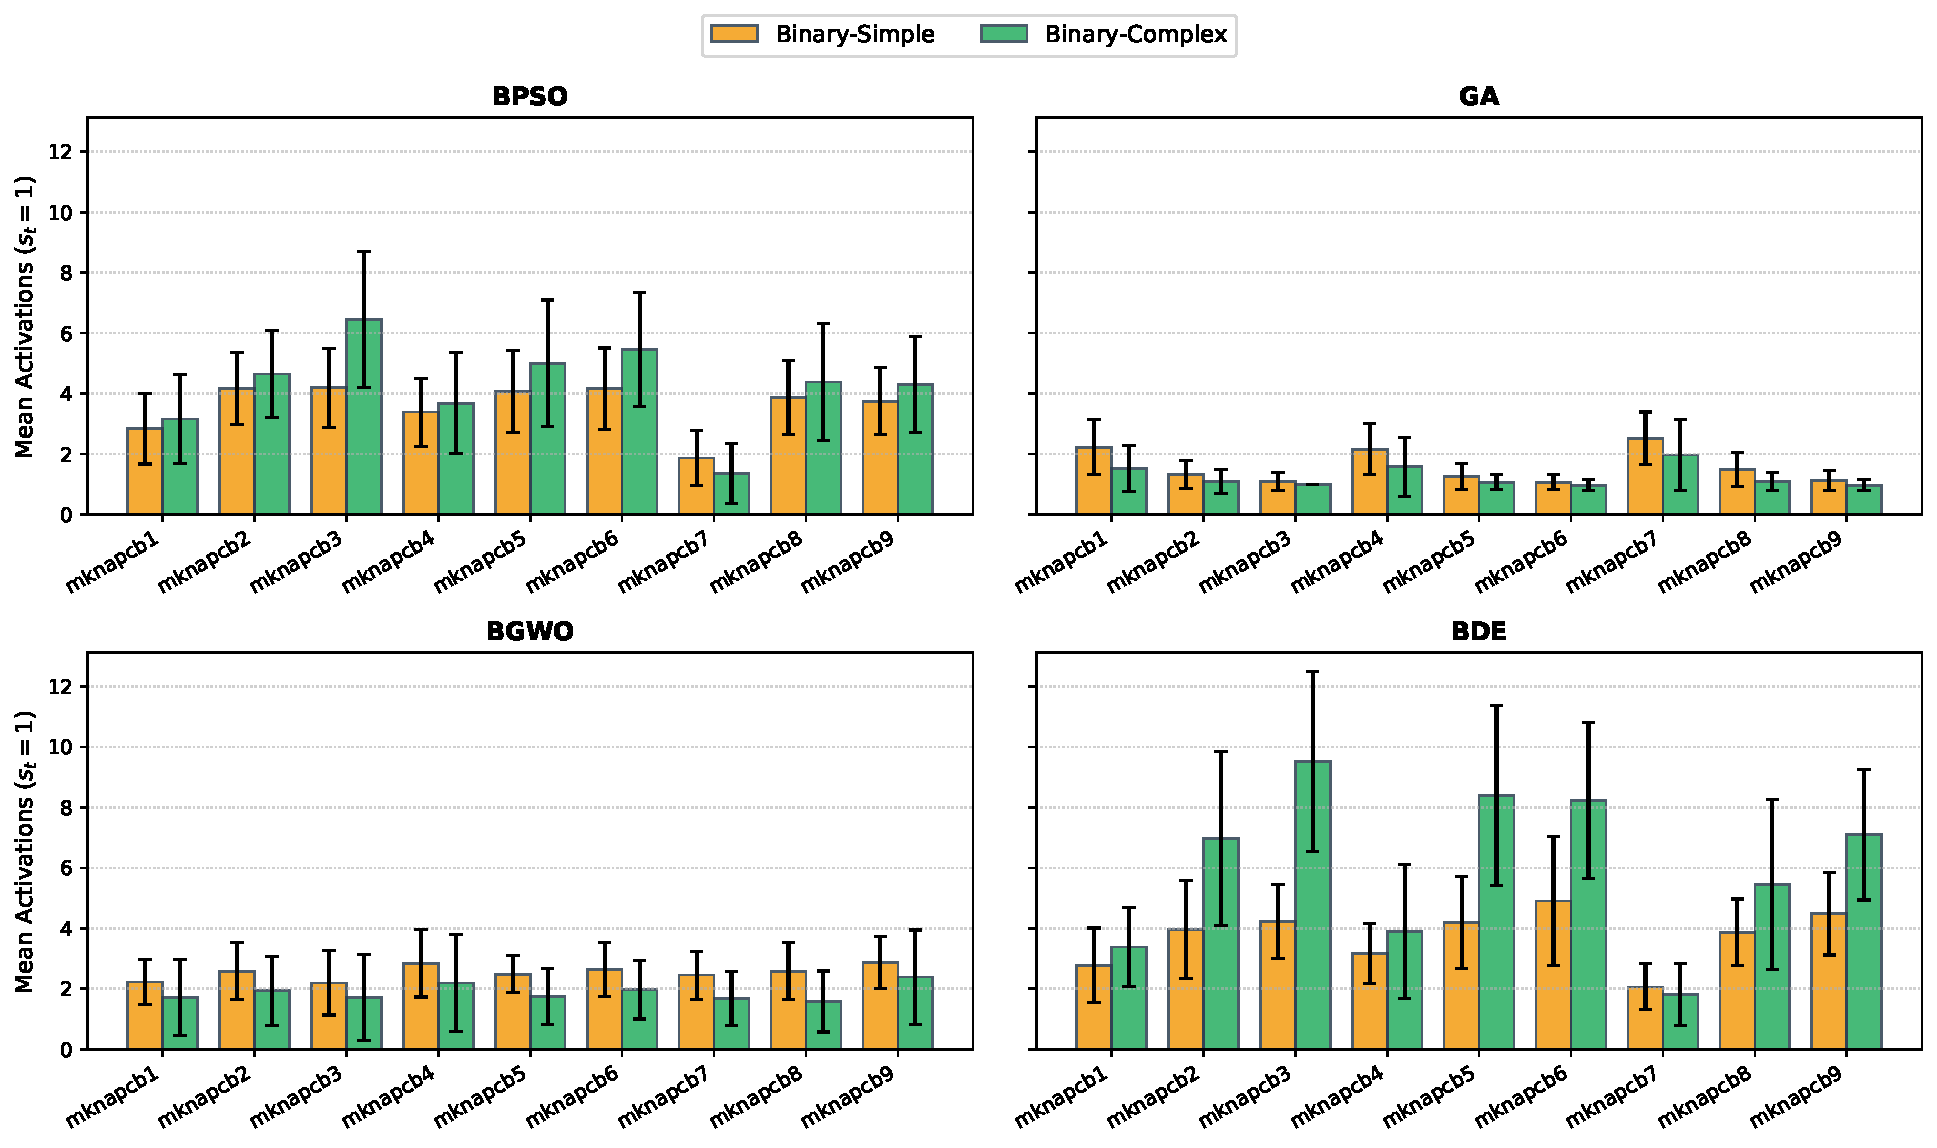
\includegraphics[width=\textwidth]{fig_dtw_activations_grid.pdf}
  \caption{Mean number of transitions to the exploration-oriented
  configuration ($s_t=1$) over 31 independent runs for Binary-Simple and
  Binary-Complex across the nine MKP benchmark instances. Error bars
  represent standard deviations.}
  \label{fig:dtw_activations}
\end{figure}

The controller behavior differs across the underlying metaheuristics and,
in several cases, between the two adaptive strategies. For BDE,
Binary-Complex produces a larger number of transitions to exploration than
Binary-Simple on several instances, with particularly pronounced differences
on \texttt{mknapcb2}, \texttt{mknapcb3}, \texttt{mknapcb5},
\texttt{mknapcb6}, and \texttt{mknapcb9}. A similar, although less
pronounced, pattern is observed for BPSO, where Binary-Complex generally
triggers more transitions to the exploration-oriented configuration than
Binary-Simple. In contrast, BGWO exhibits comparatively similar transition
counts between the two adaptive strategies across most instances, while GA
generally shows lower numbers of exploratory transitions.

These differences are noteworthy because the DDTW trajectory-analysis
parameters are kept unchanged across all metaheuristics and benchmark
instances. Thus, the observed transition patterns emerge from the interaction
between the common trajectory-driven control mechanism and the search
trajectories generated by the underlying metaheuristics, rather than from
metaheuristic-specific adjustment of the trajectory-analysis module. This
behavior provides empirical support for the ability of the proposed
framework to respond differently to the search dynamics produced by distinct
metaheuristic paradigms while retaining a common trajectory-analysis
mechanism.

The transition patterns can also be considered together with the solution
quality results. For BDE, the larger number of exploration transitions
produced by Binary-Complex occurs in several instances where the strategy
also achieves favorable solution quality relative to the fixed
configurations. Conversely, BGWO exhibits comparatively small differences
between Binary-Simple and Binary-Complex in both transition behavior and
final solution quality. These observations suggest an association between
controller activity and the response of the underlying metaheuristic.
However, they do not imply that a larger number of transitions to exploration
is inherently beneficial, since the effectiveness of a configuration change
depends on the search conditions under which it is triggered.

Overall, the controller analysis confirms that trajectory-driven adaptation
does not reduce to a fixed or uniform switching schedule. Binary-Simple
responds directly to the plateau-distance condition, whereas Binary-Complex
incorporates additional search conditions, temporal persistence, and
asymmetric switching. The resulting differences in transition patterns show
that controller complexity affects how trajectory information is translated
into configuration changes. Together with the solution-quality and
statistical results, this behavior supports the proposed use of explicit
trajectory-pattern analysis as feedback for adaptive configuration control
across different population-based metaheuristics.
%%%%%%%%%%%%%%%%%%%%%%%%%%%%%%%%%%%%%%%%%%


\section{Conclusions and Future Work}
\label{sec:conclusions}

This study investigated trajectory-driven adaptive configuration control for
population-based metaheuristics applied to the Multidimensional Knapsack
Problem (MKP). The proposed framework uses DDTW-based pattern analysis of
the recent best-so-far fitness trajectory as feedback for dynamically
switching between predefined exploration- and exploitation-oriented
configurations. Two adaptive strategies with different levels of controller
complexity, Binary-Simple and Binary-Complex, were evaluated using BPSO, GA,
BGWO, and BDE on nine benchmark instances covering different problem sizes
($n=100,250,500$) and numbers of constraints ($m=5,10,30$).

The experimental results show that the effectiveness of a fixed parameter
configuration depends on both the underlying metaheuristic and the problem
instance. Neither the exploration- nor the exploitation-oriented
configuration consistently provided the best performance across all
experimental conditions. This variability supports the motivation for
online configuration control based on information generated during the
search rather than relying exclusively on a single predefined operating
configuration.

The proposed trajectory-driven strategies were competitive across the
evaluated conditions and provided clear improvements in several
metaheuristic--instance combinations. Binary-Complex achieved the best
global mean rank ($2.22$), followed by Vanilla-Exploration ($2.44$),
Binary-Simple ($2.50$), and Vanilla-Exploitation ($2.83$). Although the
Friedman test did not identify statistically significant global differences
among the four strategies ($p=0.2474$), the pairwise analysis revealed
multiple conditions in which Binary-Complex significantly improved upon
the fixed configurations. Moreover, Binary-Complex obtained eight
statistically significant improvements over Binary-Simple and no
statistically significant losses in their direct comparison. These results
indicate that the additional search conditions, temporal persistence, and
asymmetric switching incorporated into the more elaborate controller can
provide benefits beyond the simpler reactive strategy.

The effect of trajectory-driven adaptation was nevertheless
metaheuristic-dependent. Particularly favorable results were observed for
BDE, where the adaptive strategies improved solution quality over the fixed
configurations in several benchmark instances. BPSO also showed that the
adaptive variants can remain competitive with a favorable fixed
exploration-oriented configuration while avoiding exclusive reliance on
that search profile. In contrast, GA exhibited conditions in which the
fixed exploitation-oriented configuration remained particularly strong,
while BGWO showed comparatively smaller differences among configurations.
These findings indicate that trajectory-driven control should not be
interpreted as a mechanism that guarantees improvement for every
metaheuristic and problem instance, but rather as a common feedback
principle whose effect depends on the search dynamics generated by the
underlying algorithm.

The analysis of controller behavior further showed that the same
trajectory-analysis parameters produced different switching patterns across
the four metaheuristics. Binary-Simple and Binary-Complex differed in the
number of transitions to the exploration-oriented configuration, with the
largest differences observed for selected BDE and BPSO instances. Since the
DDTW trajectory-analysis parameters were kept unchanged across algorithms
and instances, these results provide empirical evidence that the proposed
framework can translate trajectory information into different configuration
responses according to the observed search behavior. Finally, the runtime
analysis showed that DDTW-based adaptation introduces a manageable
computational overhead and that the additional decision logic of
Binary-Complex generally adds little cost relative to Binary-Simple.

The results support explicit pattern-based analysis of the search
trajectory as a viable source of feedback for online configuration control.
Rather than establishing a universally superior parameter configuration,
the proposed framework provides a common mechanism for adapting the
operating behavior of different metaheuristics according to information
extracted from their evolving convergence trajectories.


\subsection{Limitations}
\label{subsec:limitations}

Despite the encouraging results, the present study has several limitations.
First, the adaptive controller is restricted to discrete switching between
two predefined configurations representing exploration- and
exploitation-oriented search behaviors. Although this formulation provides
a clear and controlled setting for evaluating trajectory-driven adaptation,
it restricts the controller to a small set of possible operating states and
does not consider intermediate parameter configurations. Second, the trajectory-analysis mechanism relies exclusively on the recent best-so-far fitness trajectory. This provides an algorithm-independent temporal signal, but it does not explicitly capture other aspects of the search state, such as population diversity, spatial distribution, or changes in the structure of the candidate solutions. Consequently, distinct population states may potentially generate similar convergence trajectories. Third, the experimental study is restricted to the MKP and to four population-based metaheuristics. Although the same trajectory-analysis mechanism and parameterization were evaluated across different
metaheuristic paradigms and benchmark dimensions, broader conclusions
regarding cross-problem applicability require validation on additional
combinatorial optimization problems and algorithmic families.

The reference patterns and trajectory-analysis parameters were
kept fixed throughout the experimental study. This design facilitates a
controlled assessment of the proposed mechanism, but the sensitivity of the
controller to the trajectory window, reference-pattern characteristics,
percentile thresholds, and persistence parameters remains to be studied
systematically.


\subsection{Future Research Directions}
\label{subsec:future_work}

The present results suggest several directions for extending
trajectory-driven adaptive configuration control. A first direction is the
development of continuous configuration-control mechanisms in which the
trajectory information is mapped to intermediate parameter configurations
rather than exclusively triggering discrete transitions between two
predefined states. Such mechanisms could provide finer control over the
exploration--exploitation balance while preserving the trajectory-driven
feedback principle introduced in this work. On the other hand, a second direction is to enrich the characterization of the search state by combining trajectory-pattern information with complementary population-level signals. Measures of population diversity, spatial distribution, improvement rate, or other search descriptors could be integrated with the temporal information extracted from the convergence trajectory. This would enable the controller to distinguish search conditions that may exhibit similar fitness trajectories but different population dynamics.

Future work should also evaluate the framework on additional discrete and
continuous optimization problems and with other metaheuristic families.
Such experiments would allow the cross-problem applicability of
trajectory-driven control to be assessed and would help determine which
properties of the underlying search dynamics favor this form of adaptation. The trajectory-analysis principle considered here provides a basis
for investigating more general forms of search-state estimation and
algorithm-level decision making. Future extensions may use trajectory-based
search-state information not only to adapt the internal configuration of a
single metaheuristic, but also to coordinate multiple search processes,
select among alternative metaheuristics, or determine when information
should be exchanged between complementary optimization strategies. These
directions extend the role of trajectory analysis from parameter
configuration control toward broader adaptive and cooperative
metaheuristic frameworks.


%%%%%%%%%%%%%%%%%%%%%%%%%%%%%%%%%%%%%%%%%%
\vspace{6pt} 

%%%%%%%%%%%%%%%%%%%%%%%%%%%%%%%%%%%%%%%%%%
%% optional
%\supplementary{The following supporting information can be downloaded at \linksupplementary{s1}, Figure S1: title; Table S1: title; Video S1: title.}

% Only for journal Methods and Protocols:
% If you wish to submit a video article, please do so with any other supplementary material.
% \supplementary{The following supporting information can be downloaded at \linksupplementary{s1}, Figure S1: title; Table S1: title; Video S1: title. A supporting video article is available at doi: link.}

% Only used for preprtints:
% \supplementary{The following supporting information can be downloaded at the website of this paper posted on \href{https://www.preprints.org/}{Preprints.org}.}

% Only for journal Hardware:
% If you wish to submit a video article, please do so with any other supplementary material.
% \supplementary{The following supporting information can be downloaded at \linksupplementary{s1}, Figure S1: title; Table S1: title; Video S1: title.\vspace{6pt}\\
%\begin{tabularx}{\textwidth}{lll}
%\toprule
%\textbf{Name} & \textbf{Type} & \textbf{Description} \\
%\midrule
%S1 & Python script (.py) & Script of python source code used in XX \\
%S2 & Text (.txt) & Script of modelling code used to make Figure X \\
%S3 & Text (.txt) & Raw data from experiment X \\
%S4 & Video (.mp4) & Video demonstrating the hardware in use \\
%... & ... & ... \\
%\bottomrule
%\end{tabularx}
%}

%%%%%%%%%%%%%%%%%%%%%%%%%%%%%%%%%%%%%%%%%%
\authorcontributions{For research articles with several authors, a short paragraph specifying their individual contributions must be provided. The following statements should be used ``Conceptualization, X.X. and Y.Y.; methodology, X.X.; software, X.X.; validation, X.X., Y.Y. and Z.Z.; formal analysis, X.X.; investigation, X.X.; resources, X.X.; data curation, X.X.; writing---original draft preparation, X.X.; writing---review and editing, X.X.; visualization, X.X.; supervision, X.X.; project administration, X.X.; funding acquisition, Y.Y. All authors have read and agreed to the published version of the manuscript.'', please turn to the  \href{http://img.mdpi.org/data/contributor-role-instruction.pdf}{CRediT taxonomy} for the term explanation. Authorship must be limited to those who have contributed substantially to the work~reported.}

\funding{Please add: ``This research received no external funding'' or ``This research was funded by NAME OF FUNDER grant number XXX''. Check carefully that the details given are accurate and use the standard spelling of funding agency names at \url{https://search.crossref.org/funding}, any errors may affect your future funding.}

\institutionalreview{In this section, please add the Institutional Review Board Statement and approval number for studies involving humans or animals. You might choose to exclude this statement if the study did not require ethical approval. Please note that the Editorial Office might ask you for further information. Please add ``The study was conducted in accordance with the Declaration of Helsinki, and approved by the Institutional Review Board (or Ethics Committee) of NAME OF INSTITUTE (protocol code XXX and date of approval).” for studies involving humans OR ``The animal study protocol was approved by the Institutional Review Board (or Ethics Committee) of NAME OF INSTITUTE (protocol code XXX and date of approval).” for studies involving animals OR ``Ethical review and approval were waived for this study due to REASON (please provide a detailed justification).” OR ``Not applicable.” for studies not involving humans or animals.}

\informedconsent{Any research article describing a study involving humans should contain this statement. Please add ``Informed consent was obtained from all subjects involved in the study.'' OR ``Patient consent was waived due to REASON (please provide a detailed justification).'' OR ``Not applicable'' for studies not involving humans. You might also choose to exclude this statement if the study did not involve humans.

Written informed consent for publication must be obtained from participating patients who can be identified (including by the patients themselves). Please state ``Written informed consent has been obtained from the patient(s) to publish this paper.” if applicable.}

\dataavailability{We encourage all authors of articles published in MDPI journals to share their research data. In this section, please provide details regarding where data supporting reported results can be found, including links to publicly archived datasets analyzed or generated during the study. Where no new data were created, or where data are unavailable due to privacy or ethical restrictions, a statement is still required. Suggested Data Availability Statements are available in the section ``MDPI Research Data Policies” at \url{https://www.mdpi.com/ethics}.} 

%\durcstatement{Current research is limited to the [please insert a specific academic field, e.g., XXX], which is beneficial [share benefits and/or primary use] and does not pose a threat to public health or national security. Authors acknowledge the dual-use potential of the research involving xxx and confirm that all necessary precautions have been taken to prevent potential misuse. As an ethical responsibility, authors strictly adhere to relevant national and international laws about DURC. Authors advocate for responsible deployment, ethical considerations, regulatory compliance, and transparent reporting to mitigate misuse risks and foster beneficial outcomes.}

% Only for journal Nursing Reports
%\publicinvolvement{Please describe how the public (patients, consumers, carers) were involved in the research. Consider reporting against the GRIPP2 (Guidance for Reporting Involvement of Patients and the Public) checklist. If the public were not involved in any aspect of the research add: ``No public involvement in any aspect of this research''.}
%
%% Only for journal Nursing Reports
%\guidelinesstandards{Please add a statement indicating which reporting guideline was used when drafting the report. For example, ``This manuscript was drafted against the XXX (the full name of reporting guidelines and citation) for XXX (type of research) research''. A complete list of reporting guidelines can be accessed via the equator network: \url{https://www.equator-network.org/}.}
%
%% Only for journal Nursing Reports
%\useofartificialintelligence{Please describe in detail any and all uses of artificial intelligence (AI) or AI-assisted tools used in the preparation of the manuscript. This may include, but is not limited to, language translation, language editing and grammar, or generating text. Alternatively, please state that “AI or AI-assisted tools were not used in drafting any aspect of this manuscript”.}

\acknowledgments{In this section, you can acknowledge any support given that is not covered by the author contribution or funding sections. This may include administrative and technical support, or donations in kind (e.g., materials used for experiments). Where GenAI has been used for purposes such as generating text, data, or graphics, or for study design, data collection, analysis, or interpretation of data, please add ``During the preparation of this manuscript/study, the author(s) used [tool name, version information] for the purposes of [description of use]. The authors have reviewed and edited the output and take full responsibility for the content of this publication.”}

\conflictsofinterest{Declare conflicts of interest or state ``The authors declare no conflicts of interest.” Authors must identify and declare any personal circumstances or interests that may be perceived as inappropriately influencing the representation or interpretation of reported research results. Any role of the funders in the design of the study; in the collection, analyses or interpretation of data; in the writing of the manuscript; or in the decision to publish the results must be declared in this section. If there is no role, please state ``The funders had no role in the design of the study; in the collection, analyses, or interpretation of data; in the writing of the manuscript; or in the decision to publish the~results”.} 

%%%%%%%%%%%%%%%%%%%%%%%%%%%%%%%%%%%%%%%%%%
%% Optional

%% Only for journal Encyclopedia
%\entrylink{The Link to this entry published on the encyclopedia platform.}

\abbreviations{Abbreviations}{%
The following abbreviations are used in this manuscript:\\

\noindent 
\begin{tabular}{@{}ll}
MDPI & Multidisciplinary Digital Publishing Institute\\
DOAJ & Directory of open access journals\\
TLA   & Three-letter acronym\\
LD      & Linear dichroism
\end{tabular}
}


\authorcontributions{
Conceptualization and proposed approach, J.G., J.V., and  E.V.; 
methodology, J.V., L.E., and E.V.; 
software, J.V. and L.E.; 
formal analysis, E.V., J.V., and J.G.; 
investigation, E.V., J.V., and J.G.; 
validation, R.S. and J.G.; 
writing—original draft preparation, E.V. and J.V.; 
writing—review and editing, E.V., L.E. and J.V. 
All authors have read and agreed to the published version of the manuscript.
}

\funding{Emanuel Vega was supported by the Agencia Nacional de Investigación y Desarrollo (ANID) under FONDECYT Initiation Project 11261348.}

\informedconsent{{Not Applicable}}

\dataavailability{The datasets analyzed in this study are publicly available.} 

\acknowledgments{
The authors extend their appreciation to the Intelligent Industry Doctorate Program and the Doctoral Program from the School of Informatics, both from the Pontificia Universidad Católica de Valparaíso for supporting this work. Additionally, the authors extend their gratitude to the PUCV Library for providing access to essential documents and resources.
}

\conflictsofinterest{The authors declare no conflict of interest.}

%%%%%%%%%%%%%%%%%%%%%%%%%%%%%%%%%%%%%%%%%%
\appendix
\section{Supplementary Solution Quality Results}
\label{sec:appendix_tables}

This appendix reports the complete solution-quality results for the six
MKP benchmark instances not included in the representative tables presented
in Section~\ref{subsec:solution_quality}. For each metaheuristic and control
strategy, the best fitness, average final fitness, standard deviation, and
relative optimality gap over the 31 independent runs are reported.


% ============================================================
% mknapcb2: n=250, m=5
% ============================================================
\begin{table}[htbp]
  \centering
  \small
  \caption{Solution quality on \textbf{mknapcb2}
  ($n=250$, $m=5$, $f^*=59\,312$).}
  \label{tab:calidad_mknapcb2}
  \begin{tabular}{lrrrr}
    \toprule
    \textbf{MH -- Variant} &
    \textbf{Best Fitness} &
    \textbf{Average} &
    \textbf{Std.} &
    \textbf{Gap (\%)} \\
    \midrule
    BPSO -- Vanilla Exploitation & 58694 & 58320.39 & 147.28 & 1.67\% \\
    BPSO -- Vanilla Exploration  & 59000 & \textbf{58817.29} & 95.05 & \textbf{0.83\%} \\
    BPSO -- Binary-Simple        & 58947 & 58762.52 & 79.06 & 0.93\% \\
    BPSO -- Binary-Complex       & \textbf{59131} & 58765.71 & 121.62 & 0.92\% \\
    \midrule
    GA -- Vanilla Exploitation   & \textbf{59226} & \textbf{59136.48} & 61.81 & \textbf{0.30\%} \\
    GA -- Vanilla Exploration    & 58957 & 58741.10 & 104.44 & 0.96\% \\
    GA -- Binary-Simple          & 59186 & 58919.13 & 166.92 & 0.66\% \\
    GA -- Binary-Complex         & 59194 & 59030.42 & 100.03 & 0.47\% \\
    \midrule
    BGWO -- Vanilla Exploitation & 58504 & \textbf{58309.87} & 115.38 & \textbf{1.69\%} \\
    BGWO -- Vanilla Exploration  & \textbf{58686} & 58249.55 & 154.95 & 1.79\% \\
    BGWO -- Binary-Simple        & 58531 & 58269.39 & 136.12 & 1.76\% \\
    BGWO -- Binary-Complex       & \textbf{58686} & 58241.84 & 137.10 & 1.80\% \\
    \midrule
    BDE -- Vanilla Exploitation  & 59060 & 58768.68 & 185.62 & 0.92\% \\
    BDE -- Vanilla Exploration   & 59162 & 59024.42 & 68.67 & 0.48\% \\
    BDE -- Binary-Simple         & 59235 & 59093.00 & 66.73 & 0.37\% \\
    BDE -- Binary-Complex        & \textbf{59266} & \textbf{59102.74} & 81.43 & \textbf{0.35\%} \\
    \bottomrule
  \end{tabular}
\end{table}


% ============================================================
% mknapcb3: n=500, m=5
% ============================================================
\begin{table}[htbp]
  \centering
  \small
  \caption{Solution quality on \textbf{mknapcb3}
  ($n=500$, $m=5$, $f^*=120\,130$).}
  \label{tab:calidad_mknapcb3}
  \begin{tabular}{lrrrr}
    \toprule
    \textbf{MH -- Variant} &
    \textbf{Best Fitness} &
    \textbf{Average} &
    \textbf{Std.} &
    \textbf{Gap (\%)} \\
    \midrule
    BPSO -- Vanilla Exploitation & 117152 & 116590.00 & 250.28 & 2.95\% \\
    BPSO -- Vanilla Exploration  & 118393 & \textbf{118052.35} & 210.47 & \textbf{1.73\%} \\
    BPSO -- Binary-Simple        & \textbf{118421} & 117935.90 & 207.34 & 1.83\% \\
    BPSO -- Binary-Complex       & 118181 & 117890.58 & 194.54 & 1.86\% \\
    \midrule
    GA -- Vanilla Exploitation   & \textbf{120113} & \textbf{119966.16} & 58.02 & \textbf{0.14\%} \\
    GA -- Vanilla Exploration    & 118541 & 117907.84 & 301.96 & 1.85\% \\
    GA -- Binary-Simple          & 119911 & 119230.77 & 388.95 & 0.75\% \\
    GA -- Binary-Complex         & 120000 & 119870.13 & 77.47 & 0.22\% \\
    \midrule
    BGWO -- Vanilla Exploitation & 118046 & \textbf{117610.81} & 194.98 & \textbf{2.10\%} \\
    BGWO -- Vanilla Exploration  & 117961 & 117475.84 & 215.64 & 2.21\% \\
    BGWO -- Binary-Simple        & 117939 & 117502.03 & 204.21 & 2.19\% \\
    BGWO -- Binary-Complex       & \textbf{118062} & 117525.94 & 265.49 & 2.17\% \\
    \midrule
    BDE -- Vanilla Exploitation  & 118648 & 118145.74 & 369.30 & 1.65\% \\
    BDE -- Vanilla Exploration   & 119095 & 118742.87 & 244.04 & 1.15\% \\
    BDE -- Binary-Simple         & \textbf{119714} & 119199.97 & 298.48 & 0.77\% \\
    BDE -- Binary-Complex        & 119692 & \textbf{119212.68} & 293.76 & \textbf{0.76\%} \\
    \bottomrule
  \end{tabular}
\end{table}


% ============================================================
% mknapcb4: n=100, m=10
% ============================================================
\begin{table}[htbp]
  \centering
  \small
  \caption{Solution quality on \textbf{mknapcb4}
  ($n=100$, $m=10$, $f^*=23\,064$).}
  \label{tab:calidad_mknapcb4}
  \begin{tabular}{lrrrr}
    \toprule
    \textbf{MH -- Variant} &
    \textbf{Best Fitness} &
    \textbf{Average} &
    \textbf{Std.} &
    \textbf{Gap (\%)} \\
    \midrule
    BPSO -- Vanilla Exploitation & 23050 & 22888.52 & 74.28 & 0.76\% \\
    BPSO -- Vanilla Exploration  & \textbf{23055} & \textbf{22983.94} & 53.72 & \textbf{0.35\%} \\
    BPSO -- Binary-Simple        & \textbf{23055} & 22948.87 & 52.51 & 0.50\% \\
    BPSO -- Binary-Complex       & \textbf{23055} & 22968.35 & 58.21 & 0.41\% \\
    \midrule
    GA -- Vanilla Exploitation   & \textbf{23057} & 22876.87 & 90.41 & 0.81\% \\
    GA -- Vanilla Exploration    & \textbf{23057} & \textbf{22915.45} & 74.49 & \textbf{0.64\%} \\
    GA -- Binary-Simple          & \textbf{23057} & 22911.58 & 70.00 & 0.66\% \\
    GA -- Binary-Complex         & \textbf{23057} & 22910.55 & 84.55 & 0.67\% \\
    \midrule
    BGWO -- Vanilla Exploitation & 22800 & 22654.06 & 80.20 & 1.78\% \\
    BGWO -- Vanilla Exploration  & 22780 & 22645.32 & 60.10 & 1.82\% \\
    BGWO -- Binary-Simple        & 22781 & \textbf{22657.35} & 64.31 & \textbf{1.76\%} \\
    BGWO -- Binary-Complex       & \textbf{22850} & 22651.42 & 81.21 & 1.79\% \\
    \midrule
    BDE -- Vanilla Exploitation  & 23042 & 22879.74 & 101.76 & 0.80\% \\
    BDE -- Vanilla Exploration   & \textbf{23057} & 22964.84 & 58.34 & 0.43\% \\
    BDE -- Binary-Simple         & \textbf{23057} & \textbf{22970.10} & 54.17 & \textbf{0.41\%} \\
    BDE -- Binary-Complex        & \textbf{23057} & 22958.77 & 60.23 & 0.46\% \\
    \bottomrule
  \end{tabular}
\end{table}


% ============================================================
% mknapcb6: n=500, m=10
% ============================================================
\begin{table}[htbp]
  \centering
  \small
  \caption{Solution quality on \textbf{mknapcb6}
  ($n=500$, $m=10$, $f^*=117\,726$).}
  \label{tab:calidad_mknapcb6}
  \begin{tabular}{lrrrr}
    \toprule
    \textbf{MH -- Variant} &
    \textbf{Best Fitness} &
    \textbf{Average} &
    \textbf{Std.} &
    \textbf{Gap (\%)} \\
    \midrule
    BPSO -- Vanilla Exploitation & 114418 & 113745.42 & 350.35 & 3.38\% \\
    BPSO -- Vanilla Exploration  & \textbf{115347} & \textbf{114848.55} & 201.56 & \textbf{2.44\%} \\
    BPSO -- Binary-Simple        & 115128 & 114685.23 & 227.20 & 2.58\% \\
    BPSO -- Binary-Complex       & 115218 & 114689.16 & 204.68 & 2.58\% \\
    \midrule
    GA -- Vanilla Exploitation   & \textbf{117492} & \textbf{117299.23} & 112.59 & \textbf{0.36\%} \\
    GA -- Vanilla Exploration    & 115553 & 114756.71 & 323.00 & 2.52\% \\
    GA -- Binary-Simple          & 117153 & 116063.45 & 491.12 & 1.41\% \\
    GA -- Binary-Complex         & 117348 & 117010.52 & 445.41 & 0.61\% \\
    \midrule
    BGWO -- Vanilla Exploitation & \textbf{114725} & \textbf{113975.13} & 274.89 & \textbf{3.19\%} \\
    BGWO -- Vanilla Exploration  & 114446 & 113825.61 & 229.23 & 3.31\% \\
    BGWO -- Binary-Simple        & 114465 & 113822.39 & 281.92 & 3.32\% \\
    BGWO -- Binary-Complex       & 114655 & 113735.71 & 288.35 & 3.39\% \\
    \midrule
    BDE -- Vanilla Exploitation  & 116103 & 115162.87 & 511.21 & 2.18\% \\
    BDE -- Vanilla Exploration   & 116004 & 115517.26 & 238.08 & 1.88\% \\
    BDE -- Binary-Simple         & \textbf{117018} & \textbf{116215.94} & 427.61 & \textbf{1.28\%} \\
    BDE -- Binary-Complex        & 116786 & 116180.45 & 437.48 & 1.31\% \\
    \bottomrule
  \end{tabular}
\end{table}


% ============================================================
% mknapcb7: n=100, m=30
% ============================================================
\begin{table}[htbp]
  \centering
  \small
  \caption{Solution quality on \textbf{mknapcb7}
  ($n=100$, $m=30$, $f^*=21\,946$).}
  \label{tab:calidad_mknapcb7}
  \begin{tabular}{lrrrr}
    \toprule
    \textbf{MH -- Variant} &
    \textbf{Best Fitness} &
    \textbf{Average} &
    \textbf{Std.} &
    \textbf{Gap (\%)} \\
    \midrule
    BPSO -- Vanilla Exploitation & \textbf{21946} & 21722.74 & 84.37 & 1.02\% \\
    BPSO -- Vanilla Exploration  & \textbf{21946} & \textbf{21796.81} & 101.26 & \textbf{0.68\%} \\
    BPSO -- Binary-Simple        & 21840 & 21730.16 & 65.37 & 0.98\% \\
    BPSO -- Binary-Complex       & \textbf{21946} & 21771.13 & 89.79 & 0.80\% \\
    \midrule
    GA -- Vanilla Exploitation   & 21787 & 21609.06 & 75.62 & 1.54\% \\
    GA -- Vanilla Exploration    & \textbf{21946} & \textbf{21768.84} & 76.96 & \textbf{0.81\%} \\
    GA -- Binary-Simple          & \textbf{21946} & 21756.48 & 79.81 & 0.86\% \\
    GA -- Binary-Complex         & \textbf{21946} & 21756.90 & 76.52 & 0.86\% \\
    \midrule
    BGWO -- Vanilla Exploitation & \textbf{21787} & \textbf{21660.00} & 45.05 & \textbf{1.30\%} \\
    BGWO -- Vanilla Exploration  & 21682 & 21650.71 & 35.33 & 1.35\% \\
    BGWO -- Binary-Simple        & \textbf{21787} & 21648.97 & 52.08 & 1.35\% \\
    BGWO -- Binary-Complex       & \textbf{21787} & 21656.55 & 42.30 & 1.32\% \\
    \midrule
    BDE -- Vanilla Exploitation  & 21772 & 21619.39 & 59.86 & 1.49\% \\
    BDE -- Vanilla Exploration   & 21787 & \textbf{21729.84} & 47.83 & \textbf{0.98\%} \\
    BDE -- Binary-Simple         & 21874 & 21711.23 & 55.91 & 1.07\% \\
    BDE -- Binary-Complex        & \textbf{21946} & 21712.61 & 64.68 & 1.06\% \\
    \bottomrule
  \end{tabular}
\end{table}


% ============================================================
% mknapcb8: n=250, m=30
% ============================================================
\begin{table}[htbp]
  \centering
  \small
  \caption{Solution quality on \textbf{mknapcb8}
  ($n=250$, $m=30$, $f^*=56\,693$).}
  \label{tab:calidad_mknapcb8}
  \begin{tabular}{lrrrr}
    \toprule
    \textbf{MH -- Variant} &
    \textbf{Best Fitness} &
    \textbf{Average} &
    \textbf{Std.} &
    \textbf{Gap (\%)} \\
    \midrule
    BPSO -- Vanilla Exploitation & 55670 & 55263.52 & 136.79 & 2.52\% \\
    BPSO -- Vanilla Exploration  & 55916 & \textbf{55641.94} & 126.98 & \textbf{1.85\%} \\
    BPSO -- Binary-Simple        & 55781 & 55565.29 & 115.79 & 1.99\% \\
    BPSO -- Binary-Complex       & \textbf{55973} & 55615.55 & 174.69 & 1.90\% \\
    \midrule
    GA -- Vanilla Exploitation   & \textbf{56423} & \textbf{56139.06} & 141.06 & \textbf{0.98\%} \\
    GA -- Vanilla Exploration    & 55915 & 55612.58 & 168.68 & 1.91\% \\
    GA -- Binary-Simple          & 56407 & 55814.03 & 239.39 & 1.55\% \\
    GA -- Binary-Complex         & 56217 & 55982.94 & 144.62 & 1.25\% \\
    \midrule
    BGWO -- Vanilla Exploitation & 55400 & 55103.97 & 118.26 & 2.80\% \\
    BGWO -- Vanilla Exploration  & \textbf{55460} & 55078.39 & 129.34 & 2.85\% \\
    BGWO -- Binary-Simple        & 55218 & 55040.58 & 93.90 & 2.91\% \\
    BGWO -- Binary-Complex       & \textbf{55460} & \textbf{55109.03} & 141.23 & \textbf{2.79\%} \\
    \midrule
    BDE -- Vanilla Exploitation  & 56109 & 55782.52 & 187.09 & 1.61\% \\
    BDE -- Vanilla Exploration   & 56110 & 55823.10 & 149.52 & 1.53\% \\
    BDE -- Binary-Simple         & \textbf{56440} & \textbf{56044.26} & 176.34 & \textbf{1.14\%} \\
    BDE -- Binary-Complex        & 56305 & 55980.90 & 161.97 & 1.26\% \\
    \bottomrule
  \end{tabular}
\end{table}

%%%%%%%%%%%%%%%%%%%%%%%%%%%%%%%%%%%%%%%%%%
%\isPreprints{}{% This command is only used for ``preprints''.
\begin{adjustwidth}{-\extralength}{0cm}
%} % If the paper is ``preprints'', please uncomment this parenthesis.
%\printendnotes[custom] % Un-comment to print a list of endnotes

\reftitle{References}

% Please provide either the correct journal abbreviation (e.g. according to the “The list of Title Word Abbreviations” https://portal.issn.org/ltwa) or the full name of the journal. 
% Citations and references in the Supplementary Materials are permitted provided that they also appear in the reference list here. 

%=====================================
% References, variant A: external bibliography
%=====================================
 \bibliography{references}

%=====================================
% References, variant B: internal bibliography
%=====================================



% If authors have biography, please use the format below
%\section*{Short Biography of Authors}
%\bio
%{\raisebox{-0.35cm}{\includegraphics[width=3.5cm,height=5.3cm,clip,keepaspectratio]{Definitions/author1.pdf}}}
%{\textbf{Firstname Lastname} Biography of first author}
%
%\bio
%{\raisebox{-0.35cm}{\includegraphics[width=3.5cm,height=5.3cm,clip,keepaspectratio]{Definitions/author2.jpg}}}
%{\textbf{Firstname Lastname} Biography of second author}

% For the MDPI journals use author-date citation, please follow the formatting guidelines on http://www.mdpi.com/authors/references
% To cite two works by the same author: \citeauthor{ref-journal-1a} (\citeyear{ref-journal-1a}, \citeyear{ref-journal-1b}). This produces: Whittaker (1967, 1975)
% To cite two works by the same author with specific pages: \citeauthor{ref-journal-3a} (\citeyear{ref-journal-3a}, p. 328; \citeyear{ref-journal-3b}, p.475). This produces: Wong (1999, p. 328; 2000, p. 475)

%%%%%%%%%%%%%%%%%%%%%%%%%%%%%%%%%%%%%%%%%%
%% for journal Sci
%\reviewreports{\\
%Reviewer 1 comments and authors’ response\\
%Reviewer 2 comments and authors’ response\\
%Reviewer 3 comments and authors’ response
%}
%%%%%%%%%%%%%%%%%%%%%%%%%%%%%%%%%%%%%%%%%%
\PublishersNote{}
%\isPreprints{}{% This command is only used for ``preprints''.
\end{adjustwidth}
%} % If the paper is ``preprints'', please uncomment this parenthesis.
\end{document}

